\documentclass[11pt,a4paper]{article}

\usepackage[margin=23mm,headheight=15pt]{geometry}
\usepackage[T1]{fontenc}
\usepackage[utf8]{inputenc}
\usepackage{newtxtext,newtxmath}
\usepackage{microtype}
\usepackage{amsmath,mathtools,bm}
\usepackage{graphicx}
\usepackage{booktabs,tabularx,array}
\usepackage{caption}
\usepackage{enumitem}
\usepackage{float}
\usepackage{placeins}
\usepackage{xcolor}
\usepackage[most]{tcolorbox}
\usepackage{titlesec}
\usepackage{fancyhdr}
\usepackage[round,authoryear]{natbib}
\usepackage{hyperref}
\usepackage[nameinlink,capitalise,noabbrev]{cleveref}
\usepackage{listings}
\usepackage{setspace}

\graphicspath{{figures/}}

\definecolor{navy}{HTML}{1F4E79}
\definecolor{brick}{HTML}{B03A2E}
\definecolor{teal}{HTML}{2A7F62}
\definecolor{gold}{HTML}{B58900}
\definecolor{plum}{HTML}{6C5B7B}
\definecolor{softblue}{HTML}{EDF4F8}
\definecolor{softred}{HTML}{FBF0ED}
\definecolor{softgreen}{HTML}{EDF7F2}
\definecolor{softgold}{HTML}{FFF8E8}
\definecolor{softgray}{HTML}{F3F4F5}
\definecolor{ink}{HTML}{202124}

\hypersetup{
  colorlinks=true, linkcolor=navy, citecolor=teal, urlcolor=plum,
  pdftitle={Joint Score Dynamics on a Rotating Ring},
  pdfauthor={Giovanni Mantovani}
}

\titleformat{\section}{\Large\bfseries\color{navy}}{\thesection}{0.7em}{}
\titleformat{\subsection}{\large\bfseries\color{ink}}{\thesubsection}{0.65em}{}
\titleformat{\subsubsection}{\normalsize\bfseries\color{teal}}{\thesubsubsection}{0.6em}{}
\titlespacing*{\section}{0pt}{2.3ex plus 0.8ex minus 0.3ex}{1.0ex}
\titlespacing*{\subsection}{0pt}{1.9ex plus 0.6ex minus 0.2ex}{0.7ex}

\pagestyle{fancy}
\fancyhf{}
\fancyhead[L]{\small Joint score dynamics on a rotating ring}
\fancyhead[R]{\small\leftmark}
\fancyfoot[C]{\thepage}
\renewcommand{\headrulewidth}{0.3pt}
\renewcommand{\sectionmark}[1]{\markboth{\thesection\ #1}{}}

\newcommand{\R}{\mathbb{R}}
\newcommand{\E}{\mathbb{E}}
\newcommand{\N}{\mathcal{N}}
\newcommand{\KL}{D_{\mathrm{KL}}}
\newcommand{\given}{\,\vert\,}
\newcommand{\score}{\bm S}
\newcommand{\mt}{m_t}
\newcommand{\Dt}{\Delta_t}
\newcommand{\Cov}{\operatorname{Cov}}
\newcommand{\Var}{\operatorname{Var}}
\newcommand{\diag}{\operatorname{diag}}
\newcommand{\tr}{\operatorname{tr}}
\newcommand{\dd}{\,\mathrm d}
\newcommand{\e}{\mathrm e}
\newcommand{\T}{^{\mkern-1.5mu\mathsf{T}}}
\newcommand{\wrap}{\operatorname{wrap}}
\newcommand{\WN}{\operatorname{WN}}
\newcommand{\ohat}{\widehat}

\newtcolorbox{keyresult}[1][]{
  enhanced, breakable, colback=softblue, colframe=navy, boxrule=0.75pt, arc=1.5mm,
  left=2mm, right=2mm, top=1.5mm, bottom=1.5mm,
  title={#1}, colbacktitle=navy, coltitle=white, fonttitle=\bfseries}
\newtcolorbox{intuition}[1][]{
  enhanced, breakable, colback=softgreen, colframe=teal, boxrule=0.7pt, arc=1.5mm,
  left=2mm, right=2mm, top=1.5mm, bottom=1.5mm,
  title={#1}, colbacktitle=teal, coltitle=white, fonttitle=\bfseries}
\newtcolorbox{caution}[1][]{
  enhanced, breakable, colback=softred, colframe=brick, boxrule=0.7pt, arc=1.5mm,
  left=2mm, right=2mm, top=1.5mm, bottom=1.5mm,
  title={#1}, colbacktitle=brick, coltitle=white, fonttitle=\bfseries}
\newtcolorbox{definitionbox}[1][]{
  enhanced, breakable, colback=softgold, colframe=gold, boxrule=0.7pt, arc=1.5mm,
  left=2mm, right=2mm, top=1.5mm, bottom=1.5mm,
  title={#1}, colbacktitle=gold, coltitle=black!78, fonttitle=\bfseries}

% Toolbox: a self-contained derivation, numbered independently of the sections.
\newcounter{toolbox}
\renewcommand{\thetoolbox}{\arabic{toolbox}}
\newtcolorbox[use counter=toolbox]{toolbox}[1]{
  enhanced, breakable, colback=softgray, colframe=black!45, boxrule=0.6pt, arc=1.2mm,
  left=2.5mm, right=2.5mm, top=1.5mm, bottom=1.5mm,
  title={Toolbox~\thetcbcounter.\ #1},
  colbacktitle=black!48, coltitle=white, fonttitle=\bfseries}
\crefname{toolbox}{toolbox}{toolboxes}
\Crefname{toolbox}{Toolbox}{Toolboxes}

\captionsetup{font=small,labelfont=bf,labelsep=period}
\setlist[itemize]{leftmargin=1.5em,itemsep=0.2em,topsep=0.3em}
\setlist[enumerate]{leftmargin=1.7em,itemsep=0.25em,topsep=0.3em}
\setlength{\parindent}{0pt}
\setlength{\parskip}{0.5em}
\allowdisplaybreaks
\onehalfspacing

\lstset{basicstyle=\ttfamily\small, backgroundcolor=\color{softgray}, frame=single,
        rulecolor=\color{black!20}, breaklines=true, columns=fullflexible,
        showstringspaces=false}

\begin{document}
\hypersetup{pageanchor=false}

\begin{titlepage}
\thispagestyle{empty}
\vspace*{4mm}
{\Large\color{navy}\bfseries Master's thesis research note}\par
\vspace{5mm}
{\fontsize{28}{32}\selectfont\bfseries Joint Score Dynamics on a Rotating Ring}\par
\vspace{3mm}
{\Large The first board problem: from an exactly solvable surrogate\\ to the polar process}\par
\vspace{6mm}
\vspace{2mm}
\begin{center}
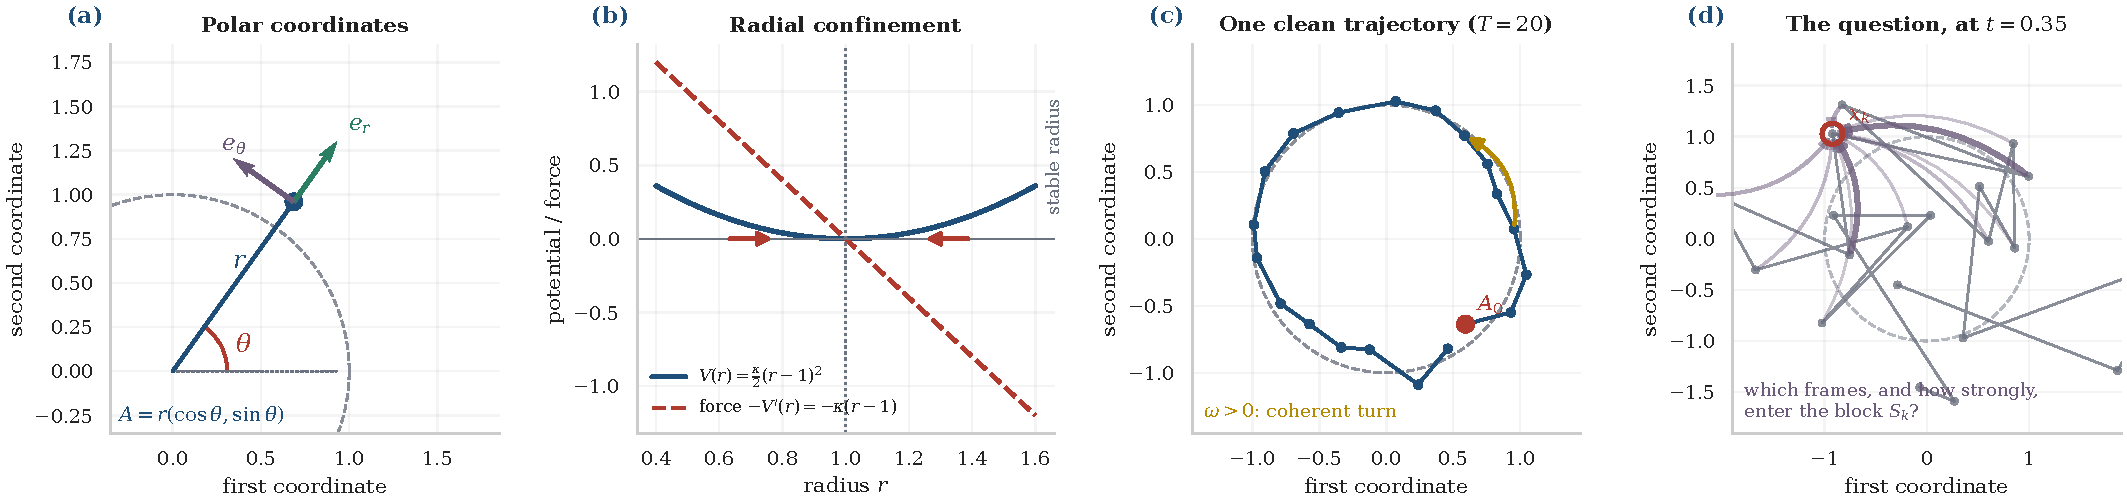
\includegraphics[width=\textwidth]{fig01_problem_setup.pdf}\\[7mm]
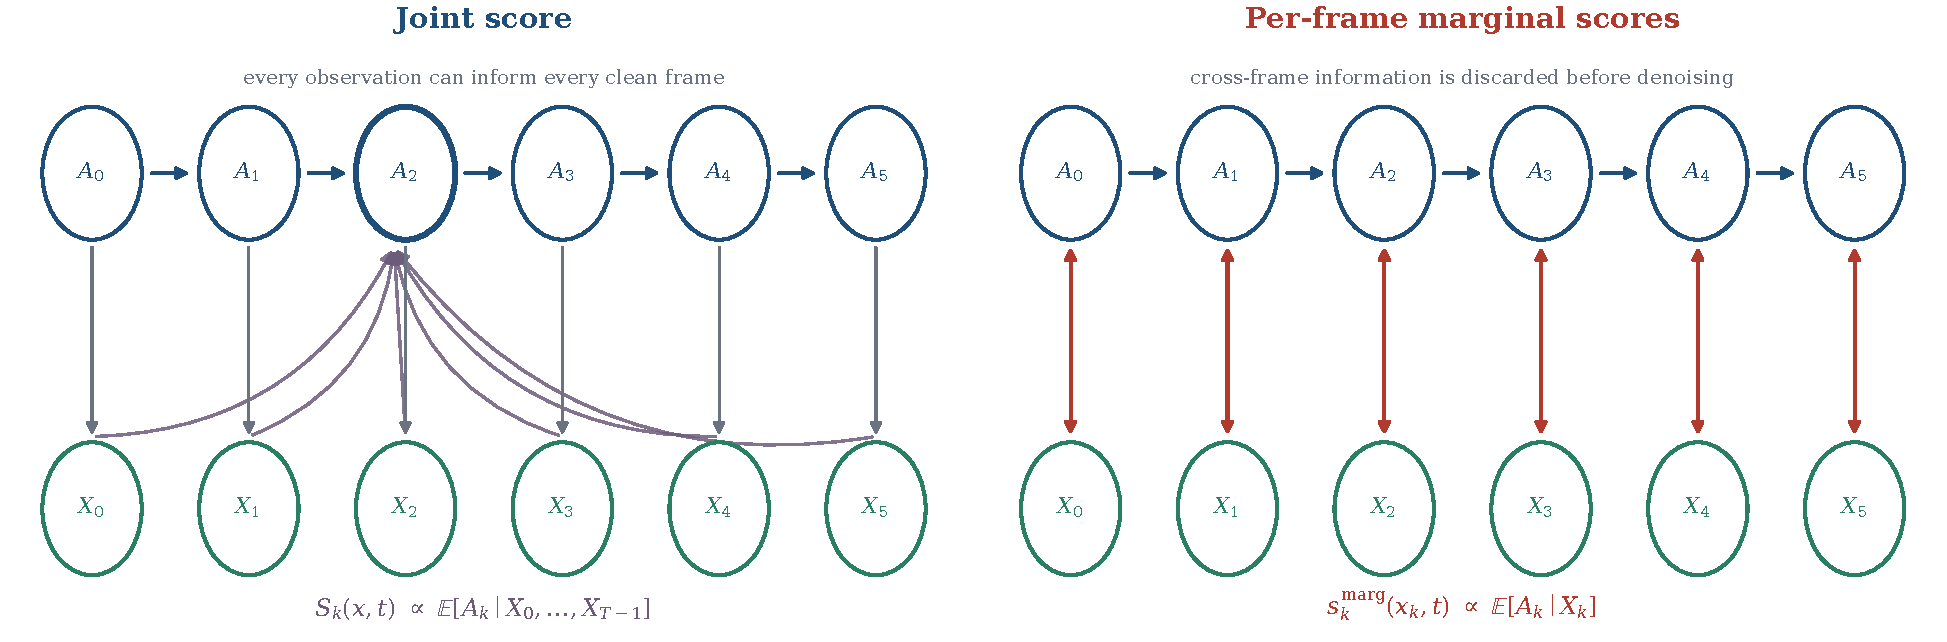
\includegraphics[width=\textwidth]{fig03_score_graphs.pdf}
\end{center}
\vfill
{\large Giovanni Mantovani}\par
{\normalsize Bocconi University --- Data Science and Business Analytics}\par
{\normalsize 26 July 2026}\par
\vspace{3mm}
{\small This note develops the first of the three problems discussed on the board with
Marc M\'ezard. It reconstructs the background it needs from first principles, derives
every identity it uses, separates the exactly solvable surrogate from the polar process
that was actually drawn, and reports what the simulations do and do not establish.}\par
\end{titlepage}

\hypersetup{pageanchor=true}
\pagenumbering{roman}

\begin{abstract}
\noindent
A dynamic object is a whole trajectory, not a collection of independent frames. This note
studies the joint diffusion score of a noisy rotating trajectory near a unit ring, and asks
how the Markov structure of the clean trajectory can be used to compute and interpret that
score. The work proceeds in two stages. A Cartesian rotating-random-walk surrogate is solved
in closed form: the known rotation is removed by an orthogonal change of coordinates, after
which the noised score is a Gaussian random-walk term plus a rank-one correction generated by
the shared ring anchor. The polar process of the board is then treated directly: its radial
and angular one-step transitions are derived from the stochastic differential equations, its
noised score is written as a posterior smoothing mean and evaluated by forward--backward
integration on a polar grid, and its response to perturbing another frame is shown to equal a
posterior covariance. A first-order expansion around one rotating branch gives an
interpretable linear-Gaussian approximation, together with an explicit statement of when it
may be used. Three diagnostics are then measured --- the absolute intensity of cross-frame
influence, its temporal reach, and the finite window needed to reproduce the score --- and a
fourth is introduced that combines reach and intensity in a single bounded number. In the one
parameter set studied here, increasing diffusion time broadens the normalised reach while
strongly reducing the absolute intensity, and tangential information travels farther than
radial information at low noise. These are measurements in a small, specific model, not
general laws.
\end{abstract}

\begin{keyresult}[What the note concludes]
\begin{enumerate}[itemsep=0.15em]
\item The clean trajectory is Markov and its clean score is local, but the score of the
      \emph{noised} joint trajectory is not local, in either model studied.
\item Clean Markovity remains useful in two concrete ways: the posterior is computable by
      repeated one-step operations rather than one integral over $2T$ latent variables, and
      any distant influence must be transmitted through a chain of local transitions, which
      gives the nonlocality a structured profile.
\item The cross-frame response of the score is exactly a posterior covariance,
      $\partial S_k/\partial x_j=-\delta_{kj}\Dt^{-1}I_2+\mt^2\Dt^{-2}\Cov(A_k,A_j\given x)$.
      This is verified numerically to $6.6\times10^{-9}$.
\item Reach, intensity, and functional receptive field are different observables and move in
      different directions with diffusion time. Reporting only a normalised correlation
      length is misleading in a finite chain.
\item At the parameters studied, tangential information reaches much farther than radial
      information at low noise. At high noise both channels are broad but weak and the score
      approaches $-x$.
\item The local linear model reproduces the score to a few per cent while the posterior stays
      within one arc of the circle; it cannot represent angular wrapping or a multimodal
      phase.
\end{enumerate}
\end{keyresult}

\setcounter{tocdepth}{2}
\tableofcontents
\clearpage
\pagenumbering{arabic}

% ============================================================================
\section{Background: the tools this note uses}\label{sec:background}
% ============================================================================

The problem below is a small one, but reading it requires stochastic calculus and a few ideas
from statistical mechanics. This section assembles exactly those, and no more. Readers who
already have them can go to \cref{sec:object}.

\subsection{Why diffusion models}\label{sec:why-diffusion}

Diffusion models are the dominant approach to generative modelling of continuous data. They
underlie the image generators deployed by the large technology companies --- latent diffusion
in Stable Diffusion \citep{rombach2022latent}, the DALL$\cdot$E and Imagen families, Adobe
Firefly --- and the same construction, with a transformer denoiser, drives video generators
such as Sora and Veo. The reach extends past media: AlphaFold~3 predicts atomic coordinates
with a diffusion module \citep{abramson2024alphafold3}, and protein design pipelines such as
RFdiffusion generate backbones the same way. What all of these share is a single mechanism:
corrupt data by a known noising process, learn to reverse it, and sample by iterated
denoising.

The mechanism is attractive for a theorist because the object being learned is not an
arbitrary function. It is the \emph{score} $\nabla_x\log p_t(x)$ of a family of smoothed
data distributions, and that family is generated by a linear stochastic differential
equation. This makes diffusion models unusually open to exact analysis, which is what the
present note exploits: in a small model the score can be computed to machine precision and
its structure inspected directly, rather than estimated from a trained network.

\subsection{Brownian motion, and why ordinary calculus fails}\label{sec:brownian}

Brown observed in 1827 that pollen grains suspended in water jitter without pause.
\citet{einstein1905brownian} explained it quantitatively: the jitter is the accumulated effect
of molecular collisions, the mean square displacement grows linearly in time,
$\E[\|X_u-X_0\|^2]=2Du$, and the diffusivity is tied to temperature and friction by
$D=k_BT/\gamma$. Wiener later constructed the limiting process rigorously; we call it
Brownian motion, or the Wiener process $B_u$, defined by $B_0=0$, independent increments,
$B_v-B_u\sim\N(0,v-u)$, and continuous paths.

The linear growth of the variance is the source of every technical difficulty that follows.
An increment scales as $\dd B\sim\sqrt{\dd u}$, which is much larger than $\dd u$ for small
$\dd u$. Brownian paths are therefore nowhere differentiable, and $\int f\dd B$ cannot be
defined the way a Riemann--Stieltjes integral is defined.

\begin{toolbox}{Total variation and quadratic variation}\label{tb:variation}
Fix $[0,u]$ and a partition $0=s_0<\cdots<s_n=u$ of mesh $\to0$. Two sums behave very
differently.

\textbf{Quadratic variation is finite.} Let
$Q_n=\sum_i(B_{s_{i+1}}-B_{s_i})^2$. Each increment is $\N(0,\Delta s_i)$ with
$\Delta s_i=s_{i+1}-s_i$, so
\[
 \E[Q_n]=\sum_i\Delta s_i=u,
 \qquad
 \Var(Q_n)=\sum_i\Var\big[(B_{s_{i+1}}-B_{s_i})^2\big]=2\sum_i(\Delta s_i)^2,
\]
using $\Var(Z^2)=2\sigma^4$ for $Z\sim\N(0,\sigma^2)$. Since
$\sum_i(\Delta s_i)^2\le\max_i\Delta s_i\cdot u\to0$, we get $Q_n\to u$ in mean square. In
shorthand,
\[
 \boxed{(\dd B_u)^2=\dd u.}
\]

\textbf{Total variation is infinite.} Let $V_n=\sum_i|B_{s_{i+1}}-B_{s_i}|$. Then
\[
 Q_n\;\le\;\Big(\max_i|B_{s_{i+1}}-B_{s_i}|\Big)\cdot V_n .
\]
Brownian paths are continuous, so the maximum increment tends to $0$ as the mesh does. If
$V_n$ stayed bounded, the right-hand side would tend to $0$, contradicting $Q_n\to u>0$.
Hence $V_n\to\infty$: Brownian paths have unbounded total variation on every interval.

\textbf{Consequence.} The Riemann--Stieltjes integral $\int f\dd g$ requires $g$ to have
bounded variation, precisely so that the limit does not depend on where inside each
subinterval $f$ is evaluated. For Brownian motion that guarantee is gone, and different
evaluation points give genuinely different limits. A convention must be chosen.
\hfill$\square$
\end{toolbox}

\begin{toolbox}{The It\^o integral, its mean, and its variance}\label{tb:ito-integral}
It\^o's convention is to evaluate the integrand at the \emph{left} endpoint of each
subinterval \citep{ito1944stochastic}:
\begin{equation}
 \int_0^u f_s\dd B_s
 :=\lim_{n\to\infty}\sum_{i}f_{s_i}\,(B_{s_{i+1}}-B_{s_i}),
 \label{eq:ito-def}
\end{equation}
the limit taken in mean square, first for piecewise-constant adapted $f$ and then extended by
density to all adapted $f$ with $\E\int_0^uf_s^2\dd s<\infty$.

The choice of the left endpoint is what makes the construction useful. Because $f_{s_i}$ is
determined by information available at time $s_i$, and the increment $B_{s_{i+1}}-B_{s_i}$ is
independent of that information with mean zero,
\begin{equation}
 \E\big[f_{s_i}(B_{s_{i+1}}-B_{s_i})\big]
 =\E\big[f_{s_i}\big]\,\E\big[B_{s_{i+1}}-B_{s_i}\big]=0 ,
 \label{eq:ito-mean}
\end{equation}
so the integral has mean zero; it is a martingale. For $i<j$ the same argument applied to the
later increment gives $\E[f_{s_i}\Delta B_i f_{s_j}\Delta B_j]=0$, so the cross terms in the
second moment vanish and
\begin{equation}
 \E\Big[\Big(\int_0^u f_s\dd B_s\Big)^2\Big]
 =\sum_i\E\big[f_{s_i}^2\big]\,\Delta s_i
 \;\longrightarrow\;
 \int_0^u\E\big[f_s^2\big]\dd s .
 \label{eq:ito-isometry}
\end{equation}
This is the \emph{It\^o isometry}. Finally, if $f$ is \emph{deterministic}, each term of
\eqref{eq:ito-def} is a fixed multiple of an independent Gaussian, so the integral is Gaussian
with mean $0$ and variance $\int_0^uf_s^2\dd s$. Every stochastic integral in this note is of
that deterministic type. \hfill$\square$
\end{toolbox}

The price of the convention is a modified chain rule. This is the single formal difference
between an ordinary differential equation and a stochastic one: an ODE
$\dot X_u=b(X_u)$ transports a point along a velocity field, and any smooth function of the
solution obeys $\dd\phi=\phi'\dd X$; an SDE
$\dd X_u=b(X_u)\dd u+\sigma(X_u)\dd B_u$ carries a term of order $\sqrt{\dd u}$, whose square
is of order $\dd u$ and therefore cannot be dropped.

\begin{toolbox}{It\^o's lemma and the product rule}\label{tb:ito-lemma}
Let $X_u$ solve $\dd X_u=b\dd u+\sigma\dd B_u$ and let $\phi(x,u)$ be twice differentiable.
Expand to second order and substitute:
\[
 \dd\phi
 =\partial_u\phi\dd u+\partial_x\phi\dd X+\tfrac12\partial_x^2\phi\,(\dd X)^2+\cdots,
 \qquad
 (\dd X)^2=b^2(\dd u)^2+2b\sigma\dd u\dd B+\sigma^2(\dd B)^2 .
\]
The It\^o multiplication table --- $(\dd u)^2=0$, $\dd u\dd B=0$,
$(\dd B)^2=\dd u$, the last being \cref{tb:variation} --- leaves
\begin{equation}
 \boxed{\;\dd\phi
 =\Big(\partial_u\phi+b\,\partial_x\phi+\tfrac{\sigma^2}{2}\partial_x^2\phi\Big)\dd u
 +\sigma\,\partial_x\phi\dd B_u .}
 \label{eq:ito-lemma}
\end{equation}
The half-second-derivative term is absent from ordinary calculus. It is why densities spread,
why the Fokker--Planck equation is second order, and why exponential substitutions in SDEs
must be checked rather than assumed.

\textbf{The case used repeatedly below.} If $\phi(x,u)=g(u)x$ is \emph{linear} in $x$ then
$\partial_x^2\phi=0$, the correction vanishes, and \eqref{eq:ito-lemma} reduces to the
familiar product rule
\begin{equation}
 \dd\big(g(u)X_u\big)=g'(u)X_u\dd u+g(u)\dd X_u .
 \label{eq:product-rule}
\end{equation}
Every integrating factor in this note is of this form, so no It\^o correction ever appears ---
but that is a fact to be verified, not assumed. \hfill$\square$
\end{toolbox}

\subsection{Langevin dynamics, Fokker--Planck, and the Boltzmann law}\label{sec:langevin}

\citet{langevin1908theorie} wrote Newton's equation for a particle in a fluid with the
collisions represented as noise,
\begin{equation}
 m\ddot X_u=-\gamma\dot X_u-V'(X_u)+\sqrt{2\gamma k_BT}\,\dot B_u .
 \label{eq:langevin-full}
\end{equation}
When friction dominates inertia, the velocity relaxes fast and can be eliminated; the
resulting \emph{overdamped} Langevin equation is a first-order SDE,
\begin{equation}
 \dd X_u=-\frac{1}{\gamma}V'(X_u)\dd u+\sqrt{2D}\dd B_u,
 \qquad D=\frac{k_BT}{\gamma},
 \label{eq:langevin-overdamped}
\end{equation}
the last identity being Einstein's relation between diffusivity, temperature and friction.

The density of $X_u$ obeys a deterministic partial differential equation. For a general SDE
$\dd X=b\dd u+\sqrt{2D}\dd B$ it is the \emph{Fokker--Planck} equation
\begin{equation}
 \partial_u p=-\nabla\cdot(bp)+D\nabla^2p ,
 \label{eq:fokker-planck}
\end{equation}
which one obtains by applying \cref{tb:ito-lemma} to a test function and integrating by parts.
For the gradient drift $b=-\nabla V/\gamma$ it can be written as a continuity equation with a
current that vanishes when $p\propto\e^{-V/(\gamma D)}$, so the stationary law is the
\emph{Boltzmann distribution}
\begin{equation}
 p_\infty(x)\;\propto\;\exp\!\Big[-\frac{V(x)}{k_BT}\Big].
 \label{eq:boltzmann}
\end{equation}
(For the full second-order equation \eqref{eq:langevin-full} the stationary law is the
Maxwell--Boltzmann density in position \emph{and} velocity, $\propto
\e^{-(V+\frac12m v^2)/k_BT}$; its position marginal is again \eqref{eq:boltzmann}.)

Two consequences matter here. First, \eqref{eq:boltzmann} closes a loop between dynamics and
equilibrium: simulating \eqref{eq:langevin-overdamped} long enough samples the Boltzmann law,
which is the basis of Langevin Monte Carlo. Second, the drift needed to do so is exactly a
score,
\begin{equation}
 \nabla\log p_\infty=-\frac{\nabla V}{k_BT} ,
\end{equation}
so \emph{knowing a score is the same as knowing how to sample}. Generative diffusion is this
observation applied to a family of distributions instead of one.

\subsection{The Ornstein--Uhlenbeck process}\label{sec:ou-intro}

Take the simplest confining potential, $V(x)=\tfrac12\|x\|^2$. Then
\eqref{eq:langevin-overdamped} becomes the \emph{Ornstein--Uhlenbeck} process
\citep{uhlenbeck1930theory},
\begin{equation}
 \dd X_t=-X_t\dd t+\sqrt2\dd W_t ,
 \label{eq:ou-intro}
\end{equation}
in the normalisation used throughout this note. It is the unique process that is
simultaneously Gaussian, Markov and stationary in continuous time, it is exactly solvable
(\cref{tb:ou-channel}), and its stationary law is the standard normal.

That last property is why diffusion models use it. The forward process needs a fixed,
parameter-free distribution to end at, so that reverse sampling can be started from something
known; $\N(0,I)$ is that distribution. The particular constants in \eqref{eq:ou-intro} give
the \emph{variance-preserving} convention \citep{song2021scorebased}: signal and noise scales
satisfy $\mt^2+\Dt=1$, so data of unit variance keep unit variance at every $t$.

\subsection{Diffusion models as non-equilibrium thermodynamics}\label{sec:thermo}

\citet{sohl2015deep} introduced the construction now called a diffusion model by explicit
analogy with non-equilibrium thermodynamics. Their forward process is a chain of small
perturbations that gradually converts a structured distribution into a simple one --- an
annealing schedule --- and the generative model is a learned reversal of that chain. The
training objective they derive is a variational bound of the same algebraic form as the work
identities of non-equilibrium statistical mechanics: the log-likelihood is bounded by an
average of log-ratios along the forward path, exactly as free-energy differences are bounded
in Jarzynski-type equalities and estimated in annealed importance sampling. The analogy is
structural rather than decorative --- it is what supplies the objective --- and it is the
historical reason the field speaks of temperature, annealing and entropy at all.

The direction of the forward process is fixed by the second law.

\begin{toolbox}{The second law for the Fokker--Planck equation}\label{tb:second-law}
Let $p_t$ evolve by \eqref{eq:fokker-planck} with gradient drift and stationary law
$p_\infty\propto\e^{-V}$ (set $D=1$, $\gamma=1$, $k_BT=1$). The relative entropy
\begin{equation}
 \mathcal F[p_t]=\KL(p_t\,\|\,p_\infty)=\int p_t\log\frac{p_t}{p_\infty}
\end{equation}
is a free energy: it is the mean energy minus the entropy, up to a constant. Differentiate,
use \eqref{eq:fokker-planck} written as
$\partial_tp=\nabla\cdot\big(p\nabla\log(p/p_\infty)\big)$, and integrate by parts:
\begin{equation}
 \frac{\dd\mathcal F}{\dd t}
 =\int\partial_tp\,\log\frac{p}{p_\infty}
 =-\int p\,\Big\|\nabla\log\frac{p}{p_\infty}\Big\|^2
 \;\le\;0 .
 \label{eq:h-theorem}
\end{equation}
The free energy decreases monotonically and the relative entropy is consumed at a rate given
by a relative Fisher information; equality holds only at $p_t=p_\infty$. This is the
H-theorem, and it is the second law for this dynamics. \hfill$\square$
\end{toolbox}

\Cref{tb:second-law} says the forward channel destroys information about the data
monotonically and irreversibly, and \eqref{eq:h-theorem} identifies the rate. The reverse
direction is not forbidden, but it is not free: it requires the score of the intermediate
laws to be supplied from outside. \citet{anderson1982reverse} makes this precise --- the
time-reversed process is again a diffusion, with a drift corrected by
$\nabla\log p_t$. The entire modelling effort of a diffusion model is the estimation of that
one object, and the entire content of this note is what that object looks like when the data
are trajectories.

\subsection{Two more tools from statistical mechanics}\label{sec:statmech-tools}

\subsubsection{Fluctuation--dissipation, and linear response}

Couple a system to a small external field $h$ conjugate to an observable $a$, so that the
Gibbs weight acquires a factor $\e^{h\cdot a}$. The partition function
$Z(h)=\int\nu(a)\e^{h\cdot a}\dd a$ is then a cumulant generating function, and
\begin{equation}
 \frac{\partial\langle a_k\rangle}{\partial h_j}
 =\frac{\partial^2\log Z}{\partial h_j\partial h_k}
 =\Cov(a_k,a_j) .
 \label{eq:static-fdt}
\end{equation}
The response to a small perturbation is a spontaneous fluctuation. In equilibrium
thermodynamics this is the fluctuation--dissipation relation --- the magnetic susceptibility
equals $\beta$ times the magnetisation variance, the heat capacity equals $\beta^2$ times the
energy variance \citep{landau1980statistical}. Susceptibilities defined this way are the
standard probe of phase transitions, and they are the tool used to detect the transitions in
the training of energy-based models discussed below \citep{bachtis2024cascade}.

\Cref{eq:static-fdt} is a \emph{static} identity between a derivative and a covariance in one
fixed measure. \Cref{sec:response-identity} shows that the response of the diffusion score to
the observed data is exactly of this form. It is not a two-time dynamical
fluctuation--dissipation theorem, and this note does not claim one.

\subsubsection{First- and second-order phase transitions}

A phase transition is a non-analyticity of the free energy in the thermodynamic limit, and its
\emph{order} is the order of the derivative that first misbehaves.

\begin{itemize}
\item At a \textbf{first-order} transition the first derivative of the free energy jumps. The
      order parameter is discontinuous, latent heat is absorbed, the two phases coexist at the
      transition, and correlation lengths stay finite.
\item At a \textbf{second-order} transition the first derivative is continuous and the second
      diverges. The order parameter grows continuously from zero, the susceptibility
      \eqref{eq:static-fdt} and the correlation length diverge, and observables acquire power
      laws.
\end{itemize}

Both appear in the statistical physics of generative models. The \emph{speciation} transition
of diffusion models --- the diffusion time at which the reverse process commits to one class
of the data rather than another --- is analysed as a symmetry-breaking transition of this kind
\citep{biroli2024dynamical,achilli2026speciation}, and the training of energy-based models has
been described as a \emph{cascade} of second-order transitions, one per direction that the
model learns, each detected by the growth of the corresponding susceptibility
\citep{bachtis2024cascade}. A related hierarchical picture is reported for images
\citep{sclocchi2025phase}.

\begin{caution}[No transition is claimed here]
The model of this note has $T=20$ frames and no thermodynamic limit is taken. Correlation
lengths that grow until they reach the length of the chain and then stop are showing a
finite-size ceiling, not a divergence. \Cref{sec:diagnostics} builds the diagnostics so that
this distinction is visible rather than hidden, and \cref{sec:measurements} reports where the
ceiling is reached.
\end{caution}

% ============================================================================
\section{The object of study, and the identities it needs}\label{sec:object}
% ============================================================================

\subsection{One trajectory is one data point}

We observe a planar trajectory at internal times
\[
 u_k=kh,\qquad k=0,1,\ldots,T-1 .
\]
The clean frame is $A_k\in\R^2$ and the complete datum is the stacked vector
\begin{equation}
 A=(A_0,A_1,\ldots,A_{T-1})\in\R^{2T} .
 \label{eq:whole-trajectory}
\end{equation}
One data point is one trajectory; the $T$ frames are correlated coordinates of that single
point, not $T$ independent samples.

A second clock, the diffusion time $t\ge0$, controls how strongly the whole vector is
corrupted. The two clocks have different roles: internal time $u_k$ describes the clean
physical dynamics, diffusion time $t$ describes the artificial noising channel of the
generative model. \Cref{fig:two-clocks} shows them acting on one trajectory.

\begin{figure}[H]
\centering
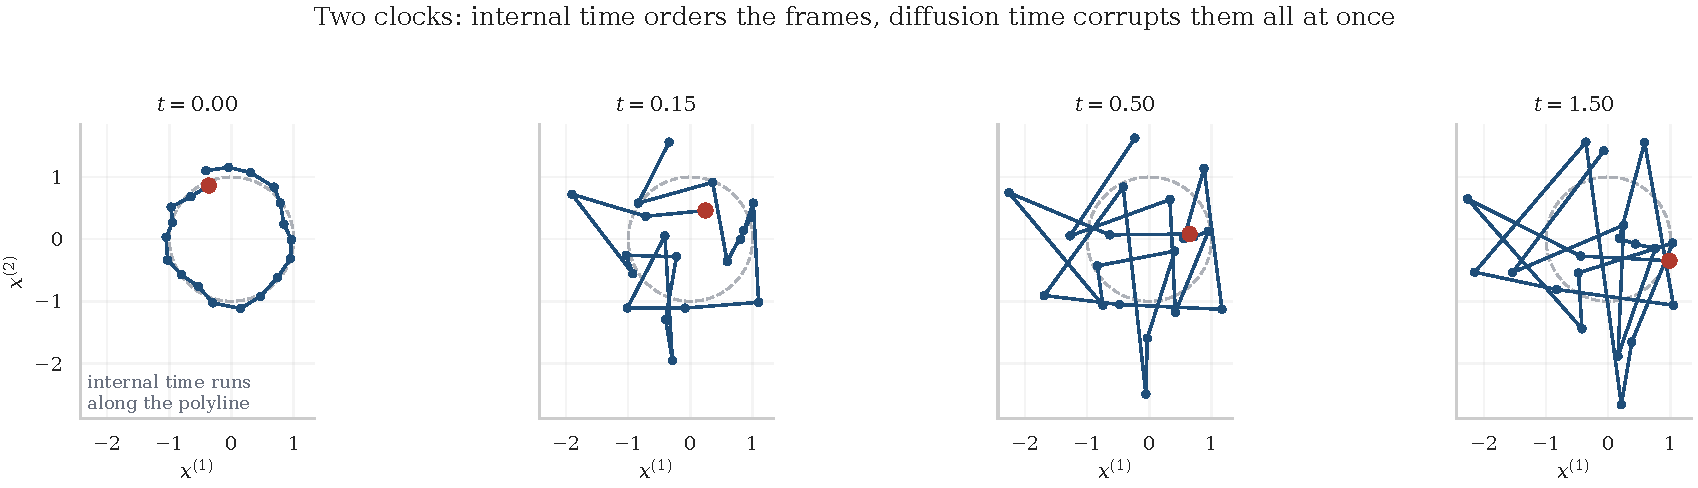
\includegraphics[width=\textwidth]{fig02_two_clocks.pdf}
\caption{The two clocks. Internal time is the ordering of the points along the polyline.
Diffusion time $t$ shrinks and corrupts every frame at once. The same standardised noise
realisation is used in all four panels, so the only difference between them is $t$.}
\label{fig:two-clocks}
\end{figure}

\subsection{Research question}

\begin{keyresult}[Research question]
How can the Markov structure of the clean rotating trajectory be exploited to compute and
understand the dynamics of the joint diffusion score?
\end{keyresult}

Four measurable subquestions make this operational.
\begin{enumerate}
\item How different is the joint score from a collection of one-frame marginal scores?
\item How strongly does the observed frame $j$ influence the score acting on frame $k$?
\item How does that influence decay with the temporal lag $|j-k|$?
\item How many neighbouring frames are needed to reproduce the full score to a given accuracy?
\end{enumerate}

\subsection{Notation}

\begin{table}[H]
\centering\small
\begin{tabularx}{\textwidth}{@{}lX@{}}
\toprule
Symbol & Meaning \\
\midrule
$k,j$ & discrete internal-time indices \\
$h$ & internal-time spacing between consecutive frames \\
$t$ & diffusion time \\
$A_k$ & clean Cartesian frame; $A$ the stacked clean trajectory \\
$X_k$ & noised Cartesian frame at diffusion time $t$ \\
$R_k,\Theta_k$ & latent radius and angle of the polar model \\
$\mt=\e^{-t}$ & signal attenuation of the variance-preserving OU channel \\
$\Dt=1-\e^{-2t}$ & variance added by that channel \\
$\score_k(x,t)$ & $k$th two-dimensional block of the joint score \\
$J_{kj}(x,t)$ & block response $\partial S_k/\partial x_j\in\R^{2\times2}$ \\
$\ell=|j-k|$ & temporal lag \\
$L$ & radius of a temporal observation window around frame $k$ \\
\bottomrule
\end{tabularx}
\end{table}

\subsection{The forward channel, solved}\label{sec:channel}

The surrogate and the polar process have different clean dynamics but the same noising
channel, so we solve it once. The forward process in diffusion time is \eqref{eq:ou-intro}
applied to the whole trajectory,
\begin{equation}
 \dd X_t=-X_t\dd t+\sqrt2\dd W_t,\qquad X_0=A ,
 \label{eq:ou-sde}
\end{equation}
with $W_t$ a Brownian motion in $\R^{2T}$.

\begin{toolbox}{Solving the variance-preserving OU channel}\label{tb:ou-channel}
\textbf{Step 1: choose the integrating factor.} Consider $\phi(x,t)=\e^tx$. It is linear in
$x$, so by \eqref{eq:product-rule} in \cref{tb:ito-lemma} no It\^o correction arises:
\[
 \dd(\e^tX_t)=\e^tX_t\dd t+\e^t\dd X_t .
\]
Substituting \eqref{eq:ou-sde} the two drift terms cancel exactly,
\begin{equation}
 \dd(\e^tX_t)
 =\e^tX_t\dd t+\e^t\big(-X_t\dd t+\sqrt2\dd W_t\big)
 =\sqrt2\,\e^t\dd W_t .
 \label{eq:ou-exact-differential}
\end{equation}
This is the whole purpose of the factor $\e^t$: it removes the drift and leaves a pure
stochastic differential, which can simply be integrated.

\textbf{Step 2: integrate from $0$ to $t$.} The left side telescopes because it is an exact
differential:
\[
 \e^tX_t-\e^0X_0=\sqrt2\int_0^t\e^s\dd W_s
 \quad\Longrightarrow\quad
 X_t=\e^{-t}A+\sqrt2\int_0^t\e^{-(t-s)}\dd W_s ,
\]
where $\e^{-t}$ has been taken inside the integral, which is legitimate because it does not
depend on the integration variable $s$.

\textbf{Step 3: identify the law of the noise term.} The integrand $\e^{-(t-s)}$ is
deterministic, so by \cref{tb:ito-integral} the integral is Gaussian, has mean zero by
\eqref{eq:ito-mean}, and by the It\^o isometry \eqref{eq:ito-isometry} has covariance
\[
 2\int_0^t\e^{-2(t-s)}\dd s
 \;\overset{v=t-s}{=}\;2\int_0^t\e^{-2v}\dd v
 =2\cdot\frac{1-\e^{-2t}}{2}
 =1-\e^{-2t} ,
\]
in each of the $2T$ coordinates independently.

\textbf{Step 4: collect.}
\begin{equation}
 \boxed{\;X_t=\mt A+\sqrt{\Dt}\,Z,\qquad
 \mt=\e^{-t},\quad \Dt=1-\e^{-2t},\quad Z\sim\N(0,I_{2T}).}
 \label{eq:ou-channel}
\end{equation}
Note $\mt^2+\Dt=1$: the channel is variance preserving, as promised in \cref{sec:ou-intro}. At
$t=0$ it is the identity; as $t\to\infty$ it forgets $A$ entirely and returns $\N(0,I_{2T})$.
\hfill$\square$
\end{toolbox}

\subsection{The joint score is a posterior denoiser}\label{sec:tweedie}

The noised density is the Gaussian smoothing of the data density,
\begin{equation}
 p_t(x)=\int p_0(a)\,\N(x;\mt a,\Dt I_{2T})\dd a .
 \label{eq:noised-density}
\end{equation}
Differentiating under the integral, and using
$\nabla_x\N(x;\mt a,\Dt I)=\N(x;\mt a,\Dt I)\,(\mt a-x)/\Dt$,
\begin{equation}
 \nabla_xp_t(x)=\int p_0(a)\,\N(x;\mt a,\Dt I)\,\frac{\mt a-x}{\Dt}\dd a .
\end{equation}
Dividing by $p_t(x)$ turns the normalised integrand into the posterior $p(a\given x)$ of the
clean trajectory given the noisy one:

\begin{keyresult}[Score--posterior identity]
\begin{equation}
 \boxed{\;\score(x,t)=\nabla_x\log p_t(x)=\frac{\mt\,\E[A\given X_t=x]-x}{\Dt}\;}
 \label{eq:score-posterior}
\end{equation}
and block by block,
\begin{equation}
 \boxed{\;S_k(x,t)
 =\frac{\mt\,\E[A_k\given X_0=x_0,\ldots,X_{T-1}=x_{T-1}]-x_k}{\Dt}\;.}
 \label{eq:block-score}
\end{equation}
\end{keyresult}

The score at frame $k$ is therefore a \emph{smoothing} estimate: it uses every observation,
past and future, to estimate one clean frame.

\subsection{Why the marginal score is a different object}\label{sec:joint-vs-marg}

The one-frame marginal score denoises frame $k$ using frame $k$ only,
\begin{equation}
 s_k^{\mathrm{marg}}(x_k,t)=\frac{\mt\,\E[A_k\given X_k=x_k]-x_k}{\Dt} ,
 \label{eq:marg-score}
\end{equation}
and subtracting it from \eqref{eq:block-score} isolates the difference exactly:
\begin{equation}
 \boxed{\;S_k(x,t)-s_k^{\mathrm{marg}}(x_k,t)
 =\frac{\mt}{\Dt}\Big(\E[A_k\given X_{0:T-1}=x]-\E[A_k\given X_k=x_k]\Big).}
 \label{eq:joint-marg-gap}
\end{equation}
The gap is precisely the extra denoising information supplied by the rest of the trajectory.
\Cref{fig:score-graphs} is the same statement as a picture: the joint score is a smoother, in
which every observation can inform every clean frame, while the product-of-marginals score
deletes all cross-frame information before denoising begins.

\begin{figure}[H]
\centering
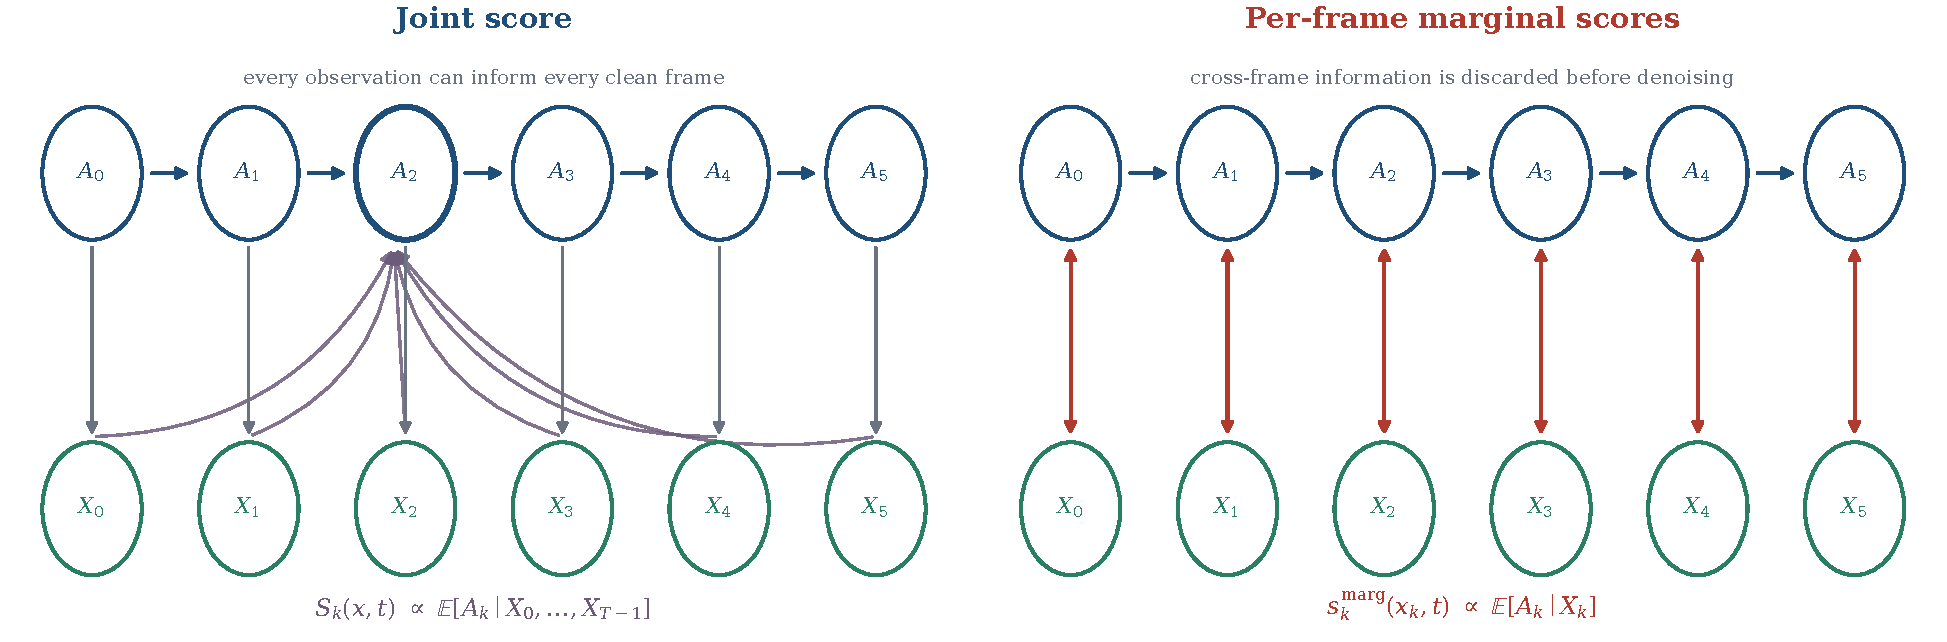
\includegraphics[width=\textwidth]{fig03_score_graphs.pdf}
\caption{The two objects compared in \eqref{eq:joint-marg-gap}, as graphical models. Clean
frames $A_k$ (blue) form a Markov chain in internal time and each emits one noisy observation
$X_k$ (green) through the channel \eqref{eq:ou-channel}. Left: computing $S_2$ requires the
posterior of $A_2$ given \emph{all} observations, so every $X_j$ has a path to $A_2$. Right:
the per-frame marginal score conditions on $X_k$ alone, which severs every cross-frame path.
The size of the difference is measured in \cref{sec:surrogate-measurements,sec:measurements}.}
\label{fig:score-graphs}
\end{figure}

\subsection{The response of the score is a posterior covariance}\label{sec:response-identity}

Question~2 of the research question asks how strongly the observation at frame $j$ influences
the score at frame $k$. The answer is an identity, and it is worth deriving slowly because
everything measured later is an instance of it.

\begin{toolbox}{From the observation as an external field to the response identity}
\label{tb:response}
\textbf{Step 1: write the posterior as a Gibbs measure with an external field.} By Bayes and
\eqref{eq:ou-channel},
\begin{align}
 p(a\given x)
 &\propto p_0(a)\exp\Big[-\frac{\|x-\mt a\|^2}{2\Dt}\Big]
 \notag\\
 &=p_0(a)\,
   \underbrace{\exp\Big[-\frac{\|x\|^2}{2\Dt}\Big]}_{\text{independent of }a}
   \exp\Big[-\frac{\mt^2}{2\Dt}\|a\|^2+\frac{\mt}{\Dt}x\T a\Big]
 \notag\\
 &\propto \underbrace{p_0(a)\exp\Big[-\frac{\mt^2}{2\Dt}\|a\|^2\Big]}_{\textstyle
   \nu(a),\ \text{independent of }x}\;\e^{\,h\T a},
 \qquad
 \boxed{\,h=\frac{\mt}{\Dt}x\,}.
 \label{eq:posterior-gibbs}
\end{align}
The expansion of $\|x-\mt a\|^2$ has produced exactly three kinds of term: one that does not
involve $a$ and is absorbed by the normalisation, one quadratic in $a$ that does not involve
$x$, and one bilinear term $x\T a$. The whole dependence on the data therefore enters through
a single vector $h$, coupled \emph{linearly} to $A$. This is the structure of
\cref{sec:statmech-tools}: the observation at frame $j$ acts as an external field
$h_j=(\mt/\Dt)x_j$ conjugate to the clean state $A_j$.

\textbf{Step 2: differentiate the log-normalisation once.} Write
$Z(h)=\int\nu(a)\e^{h\T a}\dd a$, so that $p(a\given x)=\nu(a)\e^{h\T a}/Z(h)$. Then
\begin{equation}
 \frac{\partial\log Z}{\partial h_j}
 =\frac{1}{Z}\int a_j\,\nu(a)\e^{h\T a}\dd a
 =\E[A_j\given x] .
 \label{eq:first-cumulant}
\end{equation}
$\log Z$ is the cumulant generating function of the posterior.

\textbf{Step 3: differentiate twice.} Differentiating \eqref{eq:first-cumulant} again, and
using $\partial_{h_k}\e^{h\T a}=a_k\e^{h\T a}$ together with
$\partial_{h_k}Z^{-1}=-Z^{-2}\partial_{h_k}Z$,
\begin{equation}
 \frac{\partial^2\log Z}{\partial h_k\partial h_j}
 =\E[A_kA_j\given x]-\E[A_k\given x]\E[A_j\given x]
 =\Cov(A_k,A_j\given x) .
 \label{eq:second-cumulant}
\end{equation}
Combining the last two displays, the derivative of a posterior mean with respect to the field
is a posterior covariance:
\begin{equation}
 \frac{\partial}{\partial h_j}\E[A_k\given x]=\Cov(A_k,A_j\given x) .
 \label{eq:mean-response-h}
\end{equation}

\textbf{Step 4: change variables from the field back to the data.} Since $h=(\mt/\Dt)x$ the
chain rule gives $\partial/\partial x_j=(\mt/\Dt)\,\partial/\partial h_j$, hence
\begin{equation}
 \boxed{\;\frac{\partial}{\partial x_j}\E[A_k\given x]
 =\frac{\mt}{\Dt}\Cov(A_k,A_j\given x).}
 \label{eq:mean-response}
\end{equation}

\textbf{Step 5: differentiate the score.} Apply
$\partial/\partial x_j$ to $S_k=(\mt\E[A_k\given x]-x_k)/\Dt$ from \eqref{eq:block-score}. The
first term contributes $(\mt/\Dt)$ times \eqref{eq:mean-response}; the second contributes
$-\delta_{kj}I_2/\Dt$. Therefore
\begin{equation}
 \boxed{\;J_{kj}(x,t):=\frac{\partial S_k}{\partial x_j}
 =-\frac{\delta_{kj}}{\Dt}I_2
 +\frac{\mt^2}{\Dt^2}\Cov(A_k,A_j\given X_t=x).}
 \label{eq:fdt}
\end{equation}
Here $\Cov(A_k,A_j\given x)$ is the $2\times2$ cross-covariance block between the two clean
frames under the posterior. \hfill$\square$

\textbf{Consistency check.} $J$ is the Hessian $\nabla^2\log p_t$, so it must be symmetric
under exchanging the pairs $(k,\alpha)$ and $(j,\beta)$. It is: transposing the $2\times2$
block of \eqref{eq:fdt} exchanges $A_k$ and $A_j$, and $\delta_{kj}I_2$ is symmetric.
\end{toolbox}

\begin{intuition}[What the response identity says]
For $j\ne k$ the response is proportional to a posterior cross-covariance. Perturbing a
distant observed frame changes $S_k$ if and only if the two clean states remain statistically
coupled \emph{after} conditioning on the whole noisy trajectory. The pattern of the score
Jacobian is therefore a direct map of posterior information flow, and the prefactor
$\mt^2/\Dt^2$ --- which tends to zero as $t$ grows --- is separate from that pattern. Keeping
the prefactor and the pattern apart is the point of \cref{sec:diagnostics}.
\end{intuition}

% ============================================================================
\section{Diagnostics: what to measure, and why}\label{sec:diagnostics}
% ============================================================================

Subquestions~2--4 ask about strength, reach, and sufficiency. These are three different
properties of one profile, and in the measurements below they move in different directions.
This section defines them, then builds one combined diagnostic, and states what each cannot
see.

Throughout, fix a central frame $k$ and let
\begin{equation}
 C_t(\ell)=\E_x\big[\|J_{k,k+\ell}(x,t)\|_F\big],
 \qquad \ell=0,1,\ldots,L_{\max},
 \label{eq:response-profile}
\end{equation}
be the \emph{response profile}: the average Frobenius norm of the $2\times2$ response block at
lag $\ell$, averaged over noisy trajectories and over the two sides $k\pm\ell$. The term
$C_t(0)$ is the self-response, and by \eqref{eq:fdt} it is dominated by $1/\Dt$.

\subsection{Strength: response intensity}

\begin{definitionbox}[Intensity]
\begin{equation}
 I_{\mathrm{off}}(t)=\sum_{\ell\ge1}C_t(\ell)
 \label{eq:intensity}
\end{equation}
\end{definitionbox}

This is the total amount of cross-frame response, in the units of the score Jacobian. It
answers ``how much do the other frames matter at all'', and it says nothing about where they
sit.

\subsection{Reach: three candidate lengths}

The natural first choice is an e-folding length: when the profile is close to exponential,
\[
 C_t(\ell)\approx C_t(1)\exp\!\big[-(\ell-1)/\xi^{\mathrm{exp}}\big],
\]
and $\xi^{\mathrm{exp}}$ is obtained by least squares on $\log C_t$. It is the quantity a
statistical-mechanics reading of the problem would want, because it is the finite-chain
estimate of a correlation length. It is also fragile: once the measured profile is nearly flat
the fit is ill-conditioned, and it becomes unbounded. In our measurements the fitted
$\xi^{\mathrm{exp}}_\theta$ exceeds $290$ frames in a chain of $20$ at the largest diffusion
times, which is not a length but a fit artefact. We therefore report it only in the low-noise
regime where it is meaningful (\cref{tab:exp-fits}).

A bounded alternative is the normalised range used in the first version of this study,
\begin{equation}
 \xi^{\mathrm{norm}}(t)=\sum_{\ell=1}^{L_{\max}}\frac{C_t(\ell)}{C_t(1)} ,
 \label{eq:normalised-range}
\end{equation}
which is always between $1$ and $L_{\max}$. It is stable, but it is a pure \emph{shape}
statistic: multiplying the whole profile by a constant leaves it unchanged. It therefore
cannot distinguish a strong short-range coupling from a negligible long-range one.

The third choice, and the one used from here on, is the first moment of the response mass:

\begin{definitionbox}[Weighted mean lag]
\begin{equation}
 \bar\ell(t)=\frac{\sum_{\ell\ge1}\ell\,C_t(\ell)}{\sum_{\ell\ge1}C_t(\ell)}
 =\frac{1}{I_{\mathrm{off}}(t)}\sum_{\ell\ge1}\ell\,C_t(\ell)
 \label{eq:mean-lag}
\end{equation}
\end{definitionbox}

$\bar\ell$ is the centre of mass of the cross-frame response: the average distance, in frames,
from which the response actually arrives. It is measured in frames, it is bounded by
$L_{\max}$, and --- unlike $\xi^{\mathrm{exp}}$ --- it does not assume the profile has any
particular shape. It has a known \emph{structureless ceiling}: a completely flat profile gives
$\bar\ell=(1+L_{\max})/2$, which for our $L_{\max}=10$ is $5.5$. A measured $\bar\ell$ close
to $5.5$ means that the temporal structure has been erased, not that the correlation is long.

\subsection{Both at once: a weighted reach}\label{sec:weighted-reach}

Intensity and mean lag answer complementary questions, and the product of the two is a single
number that responds to either.

\begin{definitionbox}[Weighted reach, absolute and relative]
\begin{equation}
 \Xi(t)=I_{\mathrm{off}}(t)\,\bar\ell(t)=\sum_{\ell\ge1}\ell\,C_t(\ell),
 \qquad
 \boxed{\;\widetilde\Xi(t)=\frac{\Xi(t)}{C_t(0)}\;}
 \label{eq:weighted-reach}
\end{equation}
\end{definitionbox}

Three remarks on the construction.

\begin{enumerate}
\item $\Xi$ is the unnormalised first moment of the profile. It increases if the coupling
      becomes stronger \emph{or} if it arrives from farther away, and it factorises exactly
      into ``how much'' times ``how far''. That factorisation is the reason to prefer it to an
      ad hoc combination: the two ingredients can always be read off separately.
\item Dividing by the self-response $C_t(0)$ makes it comparable across diffusion times. By
      \eqref{eq:fdt}, $C_t(0)\simeq1/\Dt$ up to the posterior variance term, so
      $\widetilde\Xi$ removes the trivial overall scale of the Jacobian and measures the reach
      of the context \emph{relative to the local term} that competes with it. It is still
      measured in frames.
\item $\widetilde\Xi$ inherits a ceiling from $\bar\ell$, so it too must be read against the
      structureless value rather than in absolute terms.
\end{enumerate}

\Cref{fig:metric-construction}(a,b) is the construction test. Four reference profiles are built
by crossing two shapes (short, long) with two amplitudes (strong, weak). By design
$\xi^{\mathrm{norm}}$ cannot separate strong from weak, $I_{\mathrm{off}}$ cannot separate
short from long, $\bar\ell$ again cannot separate strong from weak --- and $\Xi$ orders all
four. Panel (c) shows why this matters in the real measurement, and is discussed in
\cref{sec:measurements}.

\begin{figure}[H]
\centering
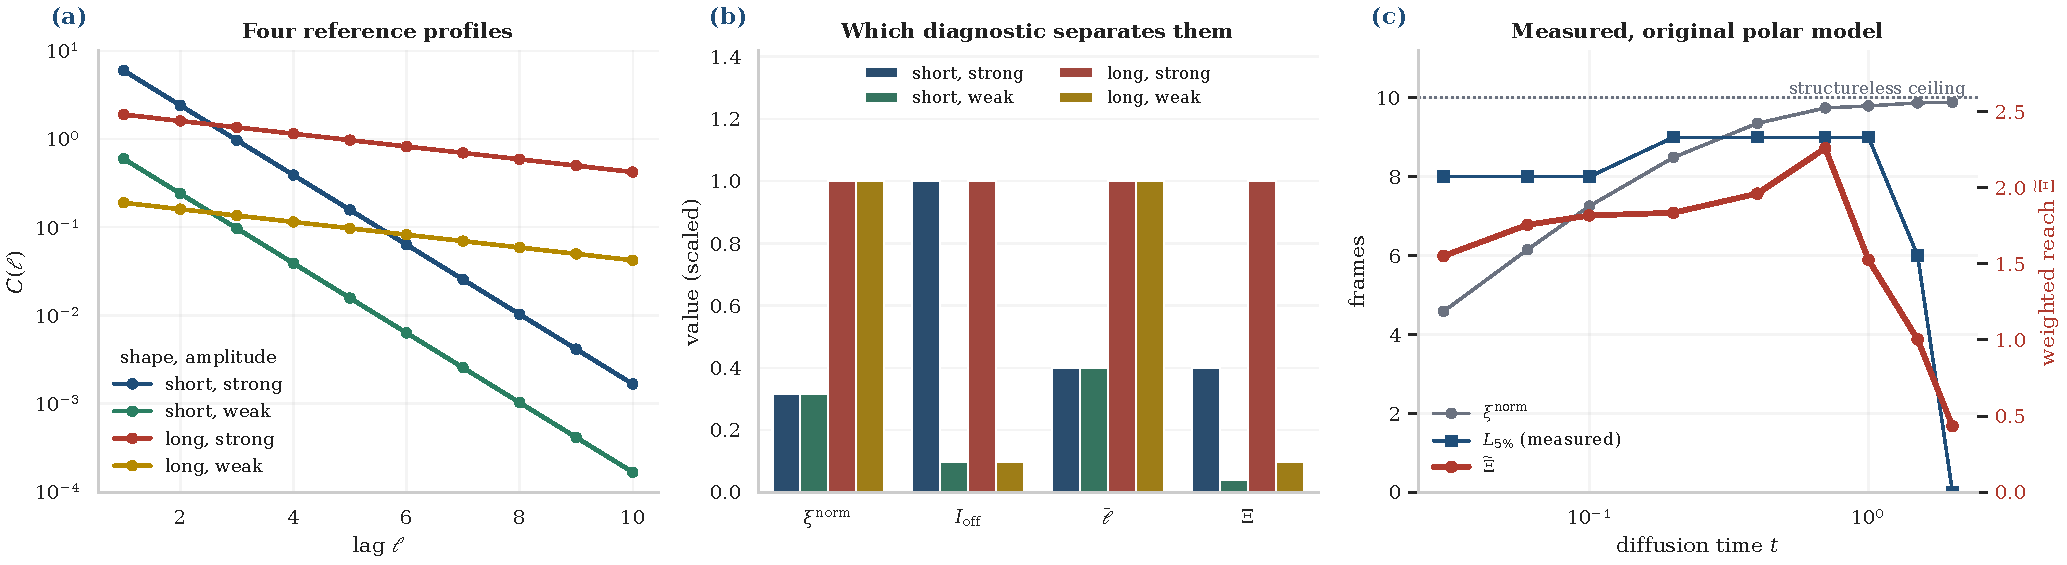
\includegraphics[width=\textwidth]{fig04_metric_construction.pdf}
\caption{Building a diagnostic that sees reach and strength together. (a) Four synthetic
reference profiles: two decay lengths crossed with two amplitudes. (b) The four diagnostics
evaluated on them, each scaled by its own maximum. $\xi^{\mathrm{norm}}$ and $\bar\ell$ are
blind to amplitude, $I_{\mathrm{off}}$ is blind to reach, and only
$\Xi=I_{\mathrm{off}}\bar\ell$ separates all four. (c) Measured in the polar model of
\cref{sec:polar}: the normalised range rises monotonically to its structureless ceiling,
whereas the weighted reach $\widetilde\Xi$ and the independently measured window radius
$L_{5\%}$ both rise and then fall.}
\label{fig:metric-construction}
\end{figure}

\subsection{Sufficiency: the functional receptive field}

Every diagnostic so far is infinitesimal --- it is built from derivatives. A more direct test
of subquestion~4 is to recompute the score from a truncated observation window
$x_{k-L:k+L}$, ignoring the rest of the trajectory entirely. Writing $S_k^{(L)}$ for that
windowed score,

\begin{definitionbox}[Window error and receptive radius]
\begin{equation}
 \varepsilon_L(t)=\left[\frac{\E\|S_k^{(L)}-S_k^{\mathrm{full}}\|^2}
                             {\E\|S_k^{\mathrm{full}}\|^2}\right]^{1/2},
 \qquad
 L_\epsilon(t)=\min\{L:\varepsilon_L(t)\le\epsilon\} .
 \label{eq:window-error}
\end{equation}
\end{definitionbox}

$L_\epsilon$ is the diagnostic with the most direct modelling meaning: it is the temporal
receptive field a network would need in order to represent the score to accuracy $\epsilon$ at
that noise level. It is also the most expensive to compute, which is why the infinitesimal
diagnostics are worth having.

\begin{caution}[What each diagnostic cannot see]
A large reach need not mean a large effect. If every off-diagonal response is tiny but nearly
equal, then $\xi^{\mathrm{norm}}$ and $\bar\ell$ both saturate at their structureless
ceilings while the total correction to the score is negligible. This is exactly what happens
at large diffusion time, where the score approaches the universal field $-x$. Conversely
$I_{\mathrm{off}}$ alone cannot tell a tightly local coupling from a diffuse one. Only the
pair, or the weighted reach that combines them, is safe to quote.
\end{caution}

% ============================================================================
\clearpage
\part{An exactly solvable surrogate}
% ============================================================================

\section{The surrogate, and the rotation as a gauge}\label{sec:surrogate}

\subsection{The model}

The surrogate keeps a ring, a coherent rotation, and statistical dependence along the
trajectory, and drops everything else:
\begin{align}
 Z_0&\sim p_\lambda(z)\propto\exp\Big[-\frac{(\|z\|-1)^2}{2\lambda}\Big],
 \label{eq:surrogate-prior}\\
 Z_{k+1}&=R_\psi Z_k+\sigma\eta_{k+1},
 \qquad\eta_{k+1}\overset{\text{iid}}{\sim}\N(0,I_2) ,
 \label{eq:surrogate-dynamics}
\end{align}
with $R_\psi$ the planar rotation through the one-frame angle $\psi$.

\begin{caution}[The surrogate is not a discretisation of the polar model]
In \eqref{eq:surrogate-dynamics} the ring acts only on $Z_0$. Later frames form a rotating
Cartesian random walk and their radial variance grows without bound. In the polar process of
\cref{sec:polar} a confining force acts at \emph{every} internal time and continually returns
the radius to one. The surrogate is a solvable companion, and its role is to make the
mechanism visible in closed form, not to approximate the board model.
\end{caution}

\subsection{The rotation matrix}\label{sec:rotation-matrix}

Because the rotation is the object we are about to remove, it is worth writing out.
\begin{equation}
 R_\psi=\begin{pmatrix}\cos\psi&-\sin\psi\\[2pt]\sin\psi&\cos\psi\end{pmatrix},
 \qquad
 R_\psi\begin{pmatrix}z^{(1)}\\z^{(2)}\end{pmatrix}
 =\begin{pmatrix}z^{(1)}\cos\psi-z^{(2)}\sin\psi\\
                 z^{(1)}\sin\psi+z^{(2)}\cos\psi\end{pmatrix}.
 \label{eq:rotation-matrix}
\end{equation}
Its columns are $R_\psi e_1=(\cos\psi,\sin\psi)$ and $R_\psi e_2=(-\sin\psi,\cos\psi)$: the two
standard basis vectors, each turned through $\psi$. They are unit vectors, since
$\cos^2\psi+\sin^2\psi=1$, and they are orthogonal, since
$\cos\psi(-\sin\psi)+\sin\psi\cos\psi=0$. In matrix form,
\begin{equation}
 R_\psi\T R_\psi=I_2,\qquad \det R_\psi=\cos^2\psi+\sin^2\psi=1,
 \qquad R_\psi\T=R_{-\psi},\qquad R_\psi R_\varphi=R_{\psi+\varphi} .
 \label{eq:rotation-orthogonal}
\end{equation}
Orthogonality is what we use: it means $R_\psi$ preserves inner products and hence lengths,
\begin{equation}
 \|R_\psi z\|^2=(R_\psi z)\T(R_\psi z)=z\T R_\psi\T R_\psi z=z\T z=\|z\|^2 .
 \label{eq:rotation-isometry}
\end{equation}
\Cref{fig:rotation} shows the three facts side by side.

\begin{figure}[H]
\centering
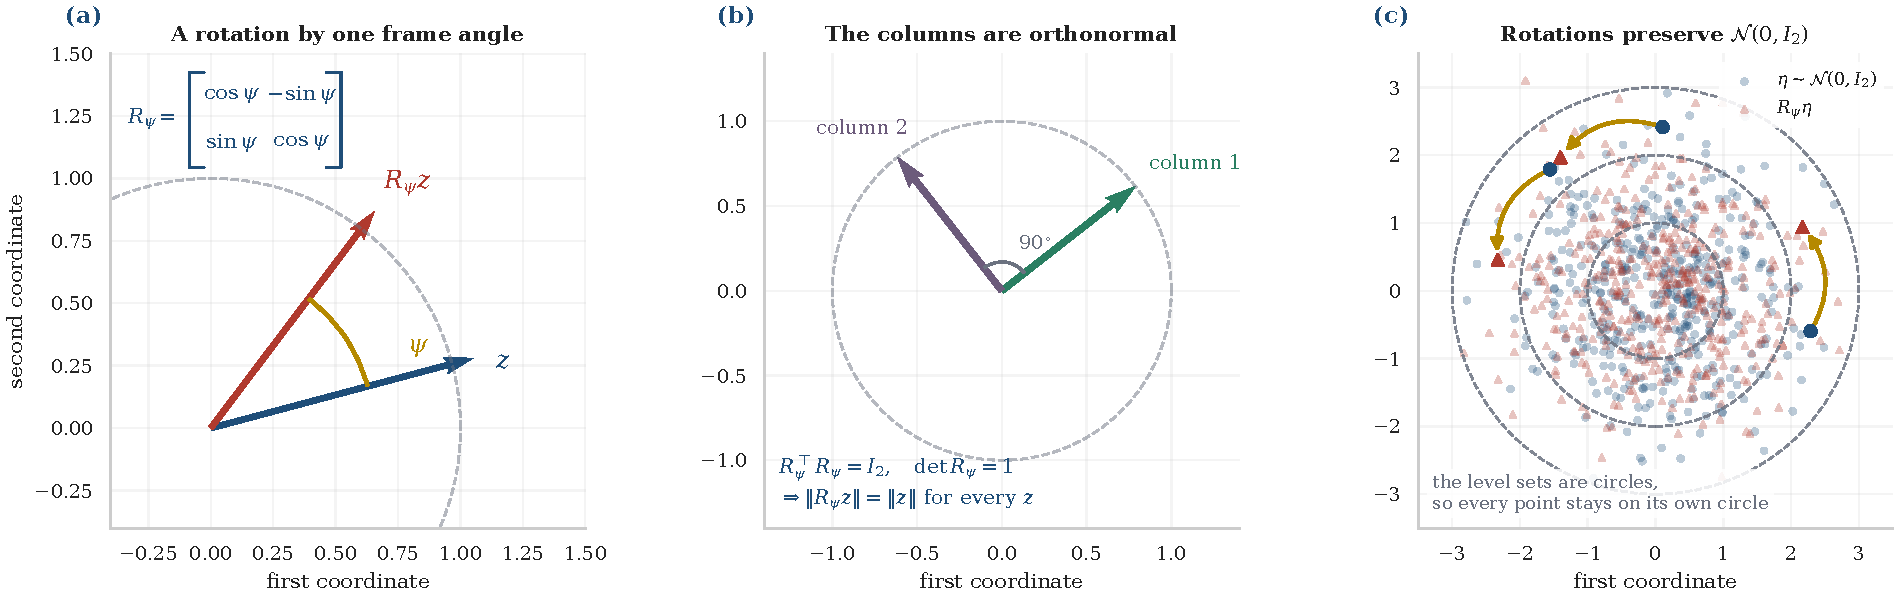
\includegraphics[width=\textwidth]{fig05_rotation.pdf}
\caption{The rotation matrix. (a) $R_\psi$ turns every vector through the same angle $\psi$
without changing its length. (b) Its columns are the rotated standard basis: unit vectors at
right angles, which is the statement $R_\psi\T R_\psi=I_2$. (c) The standard isotropic
Gaussian is unchanged, because its level sets are circles centred at the origin and a rotation
maps each circle to itself; three sample points and their images are highlighted.}
\label{fig:rotation}
\end{figure}

\subsection{Rotations preserve the standard isotropic Gaussian}\label{sec:rotation-gaussian}

This small lemma is used twice below, so we prove it twice --- once by covariance and once by
density, because the two arguments illuminate different things.

\emph{By covariance.} Let $\eta\sim\N(0,I_2)$ and $\tilde\eta=R\eta$ with $R$ orthogonal. A
linear map of a Gaussian is Gaussian, so $\tilde\eta$ is determined by its first two moments:
\begin{equation}
 \E[\tilde\eta]=R\,\E[\eta]=0,
 \qquad
 \Cov(\tilde\eta)=R\,\Cov(\eta)\,R\T=R\,I_2\,R\T=RR\T=I_2 .
\end{equation}
Hence $\tilde\eta\sim\N(0,I_2)$: the same law, not merely a similar one.

\emph{By density.} The density $p(z)=(2\pi)^{-1}\e^{-\|z\|^2/2}$ depends on $z$ only through
$\|z\|$. Under $z\mapsto Rz$ the change-of-variables formula gives the density
$p(R^{-1}z)\,|\det R^{-1}|$, and both factors are unchanged: $\|R^{-1}z\|=\|z\|$ by
\eqref{eq:rotation-isometry}, and $|\det R^{-1}|=1$ by \eqref{eq:rotation-orthogonal}. This is
the version drawn in \cref{fig:rotation}(c): the level sets are circles, and a rotation slides
each circle along itself.

The isotropy is essential. A rotation would \emph{not} preserve $\N(0,\Sigma)$ for general
$\Sigma$, and it is only because the innovation in \eqref{eq:surrogate-dynamics} and the
channel \eqref{eq:ou-channel} are both isotropic that the reduction below is exact.

\subsection{The gauge transformation}\label{sec:gauge}

\begin{definitionbox}[De-rotation]
\begin{equation}
 Y_k=R_{-k\psi}Z_k
 \label{eq:derotation}
\end{equation}
\end{definitionbox}

$Y_k$ is the trajectory as seen by an observer who turns with it: frame $k$ is rotated
\emph{back} by the total angle $k\psi$ accumulated up to that frame. Substituting
\eqref{eq:surrogate-dynamics} and using the composition rule
\eqref{eq:rotation-orthogonal},
\begin{align}
 Y_{k+1}
 &=R_{-(k+1)\psi}\big(R_\psi Z_k+\sigma\eta_{k+1}\big)
 \notag\\
 &=\underbrace{R_{-(k+1)\psi}R_\psi}_{=R_{-k\psi}}Z_k
   +\sigma R_{-(k+1)\psi}\eta_{k+1}
 \notag\\
 &=Y_k+\sigma\widetilde\eta_{k+1},
 \qquad \widetilde\eta_{k+1}:=R_{-(k+1)\psi}\eta_{k+1} .
\end{align}
By \cref{sec:rotation-gaussian} each $\widetilde\eta_{k+1}\sim\N(0,I_2)$, and they remain
independent because each is a fixed linear map of a different independent $\eta$. The rotation
has vanished:

\begin{keyresult}[Gauge-reduced surrogate]
\begin{equation}
 \boxed{Y_{k+1}=Y_k+\sigma\widetilde\eta_{k+1},
 \qquad \widetilde\eta_{k+1}\overset{\text{iid}}{\sim}\N(0,I_2).}
 \label{eq:gauged-rw}
\end{equation}
\end{keyresult}

\paragraph{Why ``gauge''.} The term is borrowed from physics, where a gauge transformation is a
change of description that leaves the physics untouched and can be chosen to simplify the
equations. Here \eqref{eq:derotation} is a known, exactly invertible, orthogonal change of
coordinates. It removes no information and introduces none: the two descriptions are the same
problem in different frames, and we are free to work in whichever is easier. That is the sense
in which the rotation ``costs no statistical difficulty''. It would not be true of an
\emph{unknown} $\psi$, which is a genuine latent variable --- see \cref{sec:limitations}.

Stacking the per-frame rotations into one $2T\times2T$ matrix,
\begin{equation}
 U_\psi=\diag\big(I_2,\,R_{-\psi},\,R_{-2\psi},\ldots,R_{-(T-1)\psi}\big),
 \qquad y=U_\psi z .
 \label{eq:U-psi}
\end{equation}

\begin{keyresult}[$U_\psi$ is orthogonal, and how the score transforms]
$U_\psi$ is block diagonal with orthogonal blocks, so
\begin{equation}
 U_\psi\T U_\psi
 =\diag\big(I_2\T I_2,\,R_{-\psi}\T R_{-\psi},\ldots\big)
 =\diag(I_2,\ldots,I_2)=I_{2T},
 \qquad
 \det U_\psi=\prod_{k}\det R_{-k\psi}=1 .
 \label{eq:U-orthogonal}
\end{equation}
Consequently, writing $p_t^{(0)}$ and $S^{(0)}$ for the $\psi=0$ quantities,
\begin{equation}
 \boxed{\;p_t(z\given\psi)=p_t^{(0)}(U_\psi z),
 \qquad
 S_\psi(z,t)=U_\psi\T\,S^{(0)}(U_\psi z,t).}
 \label{eq:gauge-score}
\end{equation}
\end{keyresult}

Both halves of \eqref{eq:gauge-score} deserve a line of proof, since they are the reason the
whole of Part~I is computable.

\emph{The density.} Apply $U_\psi$ to the channel \eqref{eq:ou-channel}:
$U_\psi X=\mt U_\psi A+\sqrt{\Dt}\,U_\psi Z$, and $U_\psi Z\sim\N(0,U_\psi U_\psi\T)=\N(0,I)$
by \eqref{eq:U-orthogonal} and \cref{sec:rotation-gaussian}. So $U_\psi X$ has exactly the law
of the noised $\psi=0$ trajectory --- the de-rotation commutes with the channel, which is the
content of \cref{fig:gauge}. For the densities, $Z=U_\psi\T Y$ gives
$p_t(z\given\psi)=p^{(0)}_t(U_\psi z)\,|\det U_\psi|=p^{(0)}_t(U_\psi z)$, the Jacobian factor
being $1$.

\emph{The score.} Differentiate the first identity with the chain rule. In components, with
$y=U_\psi z$, so that $\partial y_b/\partial z_a=(U_\psi)_{ba}$,
\begin{equation}
 \frac{\partial}{\partial z_a}\log p_t^{(0)}(U_\psi z)
 =\sum_b(U_\psi)_{ba}\,
  \big(\nabla\log p_t^{(0)}\big)_b(U_\psi z)
 =\big[U_\psi\T S^{(0)}(U_\psi z,t)\big]_a .
\end{equation}
The transpose is not cosmetic: a score is a gradient, so it transforms with $U_\psi\T$, while
a point transforms with $U_\psi$. Since $U_\psi\T=U_\psi^{-1}$ here, the recipe is simply:
\emph{de-rotate the data, solve the non-rotating problem, rotate the score back.}

\begin{figure}[H]
\centering
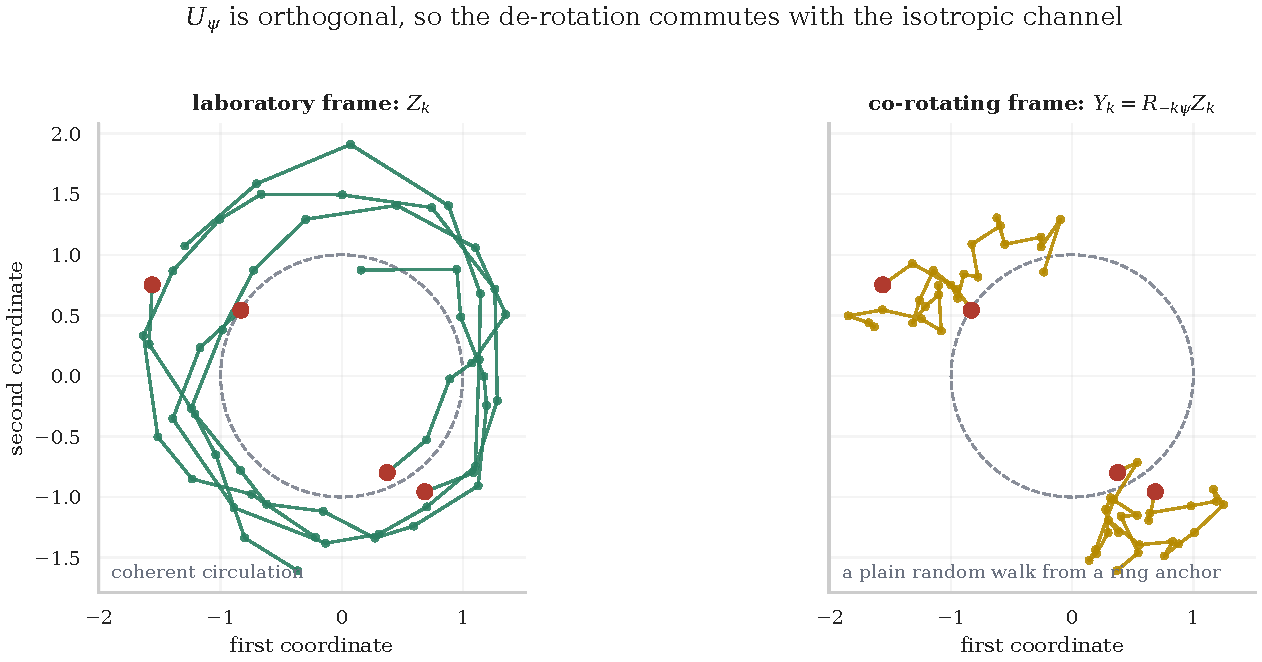
\includegraphics[width=0.86\textwidth]{fig06_gauge.pdf}
\caption{The gauge, on four trajectories ($T=14$, $\sigma=0.16$, $\psi=2\pi/14$; large dots
mark $k=0$). Left: the data, coherently circulating. Right: the same trajectories after
$U_\psi$. The circulation is gone and a random walk anchored on the ring remains. Because
$U_\psi$ is orthogonal it commutes with the isotropic channel, so the reduction is exact at
every diffusion time; the round trip is verified to machine precision
(\cref{tab:validation}).}
\label{fig:gauge}
\end{figure}

\subsection{Unrolling the recursion}\label{sec:unroll}

\Cref{eq:gauged-rw} is a random walk, and it is worth writing the first few steps explicitly
because the resulting structure --- one shared anchor plus accumulated noise --- is what makes
the model solvable.
\begin{align}
 Y_1&=Y_0+\sigma\widetilde\eta_1,\notag\\
 Y_2&=Y_1+\sigma\widetilde\eta_2=Y_0+\sigma(\widetilde\eta_1+\widetilde\eta_2),\notag\\
 Y_3&=Y_2+\sigma\widetilde\eta_3
     =Y_0+\sigma(\widetilde\eta_1+\widetilde\eta_2+\widetilde\eta_3),
 \qquad\text{and so on.}\notag
\end{align}
Formally, sum the increments and let the intermediate terms cancel:
\begin{equation}
 Y_k-Y_0=\sum_{r=1}^{k}\big(Y_r-Y_{r-1}\big)=\sigma\sum_{r=1}^{k}\widetilde\eta_r ,
\end{equation}
a telescoping sum in which every $Y_r$ with $0<r<k$ appears once with each sign. Hence

\begin{keyresult}[Shared anchor plus accumulated noise]
\begin{equation}
 \boxed{\;Y_k=A+\sigma\sum_{r=1}^{k}\widetilde\eta_r,
 \qquad A:=Y_0\sim p_\lambda,\qquad k=0,\ldots,T-1\;}
 \label{eq:rw-anchor}
\end{equation}
(the empty sum at $k=0$ being zero).
\end{keyresult}

Every frame contains the \emph{same} random anchor $A$, drawn once on the ring, plus a
partial sum of independent innovations. The anchor is a single two-dimensional variable shared
by all $T$ frames, and it is the only non-Gaussian ingredient in the model.

\section{The clean law and the exact noised score}\label{sec:surrogate-score}

\subsection{Clean joint density and clean score}

From \eqref{eq:gauged-rw} the clean law in the co-rotating frame factorises over the ring prior
and the one-step transitions,
\begin{equation}
 p_0(y_0,\ldots,y_{T-1})
 =p_\lambda(y_0)\prod_{k=0}^{T-2}\N(y_{k+1};y_k,\sigma^2I_2),
 \label{eq:surrogate-joint}
\end{equation}
so that
\begin{equation}
 \log p_0(y)
 =-\frac{(\|y_0\|-1)^2}{2\lambda}
 -\frac{1}{2\sigma^2}\sum_{k=0}^{T-2}\|y_{k+1}-y_k\|^2+\text{const} .
 \label{eq:surrogate-logdensity}
\end{equation}

Differentiating \eqref{eq:surrogate-logdensity} is elementary but instructive, so we do it in
full. For the ring term, use $\nabla_y\|y\|=y/\|y\|$:
\begin{equation}
 \nabla_{y_0}\Big[-\frac{(\|y_0\|-1)^2}{2\lambda}\Big]
 =-\frac{\|y_0\|-1}{\lambda}\cdot\frac{y_0}{\|y_0\|}
 =\frac{1-\|y_0\|}{\lambda}\cdot\frac{y_0}{\|y_0\|} ,
 \label{eq:ring-score}
\end{equation}
which points inward when $\|y_0\|>1$ and outward when $\|y_0\|<1$.

For the transition terms, the key observation is a counting one: \emph{an interior $y_k$
appears in exactly two summands of \eqref{eq:surrogate-logdensity}}, namely the edge
$(k-1,k)$ that arrives at it and the edge $(k,k+1)$ that leaves it. Differentiating each,
\begin{align}
 \nabla_{y_k}\Big[-\tfrac{1}{2\sigma^2}\|y_k-y_{k-1}\|^2\Big]
 &=-\frac{y_k-y_{k-1}}{\sigma^2}
 &&\text{(the incoming edge),}
 \label{eq:edge-in}\\
 \nabla_{y_k}\Big[-\tfrac{1}{2\sigma^2}\|y_{k+1}-y_k\|^2\Big]
 &=+\frac{y_{k+1}-y_k}{\sigma^2}
 &&\text{(the outgoing edge),}
 \label{eq:edge-out}
\end{align}
and adding them,
\begin{equation}
 -\frac{y_k-y_{k-1}}{\sigma^2}+\frac{y_{k+1}-y_k}{\sigma^2}
 =\frac{y_{k-1}-2y_k+y_{k+1}}{\sigma^2} .
\end{equation}
The boundary frames have only one incident edge each, and $y_0$ additionally carries
\eqref{eq:ring-score}. Collecting:

\begin{keyresult}[Clean score of the gauged surrogate]
\begin{align}
 S_0(y,0)&=\frac{1-\|y_0\|}{\lambda}\frac{y_0}{\|y_0\|}+\frac{y_1-y_0}{\sigma^2},
 \label{eq:clean-score-0}\\
 S_k(y,0)&=\frac{y_{k-1}-2y_k+y_{k+1}}{\sigma^2},\qquad 1\le k\le T-2,
 \label{eq:clean-score-k}\\
 S_{T-1}(y,0)&=\frac{y_{T-2}-y_{T-1}}{\sigma^2}.
 \label{eq:clean-score-T}
\end{align}
\end{keyresult}

\Cref{eq:clean-score-k} is a discrete second derivative --- a discrete Laplacian along
internal time. Three consequences are worth stating, because they are what the noised score
will destroy.

\begin{enumerate}
\item \textbf{It is strictly local.} $S_k$ involves $y_{k-1},y_k,y_{k+1}$ and nothing else.
      Each interior block measures how far frame $k$ deviates from the average of its two
      neighbours: it is a curvature, or an acceleration, along the path.
\item \textbf{It vanishes on the model's own solution.} A second difference is zero on any
      straight line in the co-rotating frame. A trajectory that rotates perfectly at radius
      exactly $1$ maps under \eqref{eq:derotation} to a \emph{constant} $Y_k$, for which every
      second difference vanishes and, since $\|y_0\|=1$, the ring term \eqref{eq:ring-score}
      vanishes too. The clean score is then exactly zero. This is checked numerically and is
      exact to machine zero (\cref{tab:validation}).
\item \textbf{Only the first frame feels the ring.} The anchor enters
      \eqref{eq:clean-score-0} alone; the rest of the trajectory knows about the ring only
      indirectly, through the chain.
\end{enumerate}

\begin{figure}[H]
\centering
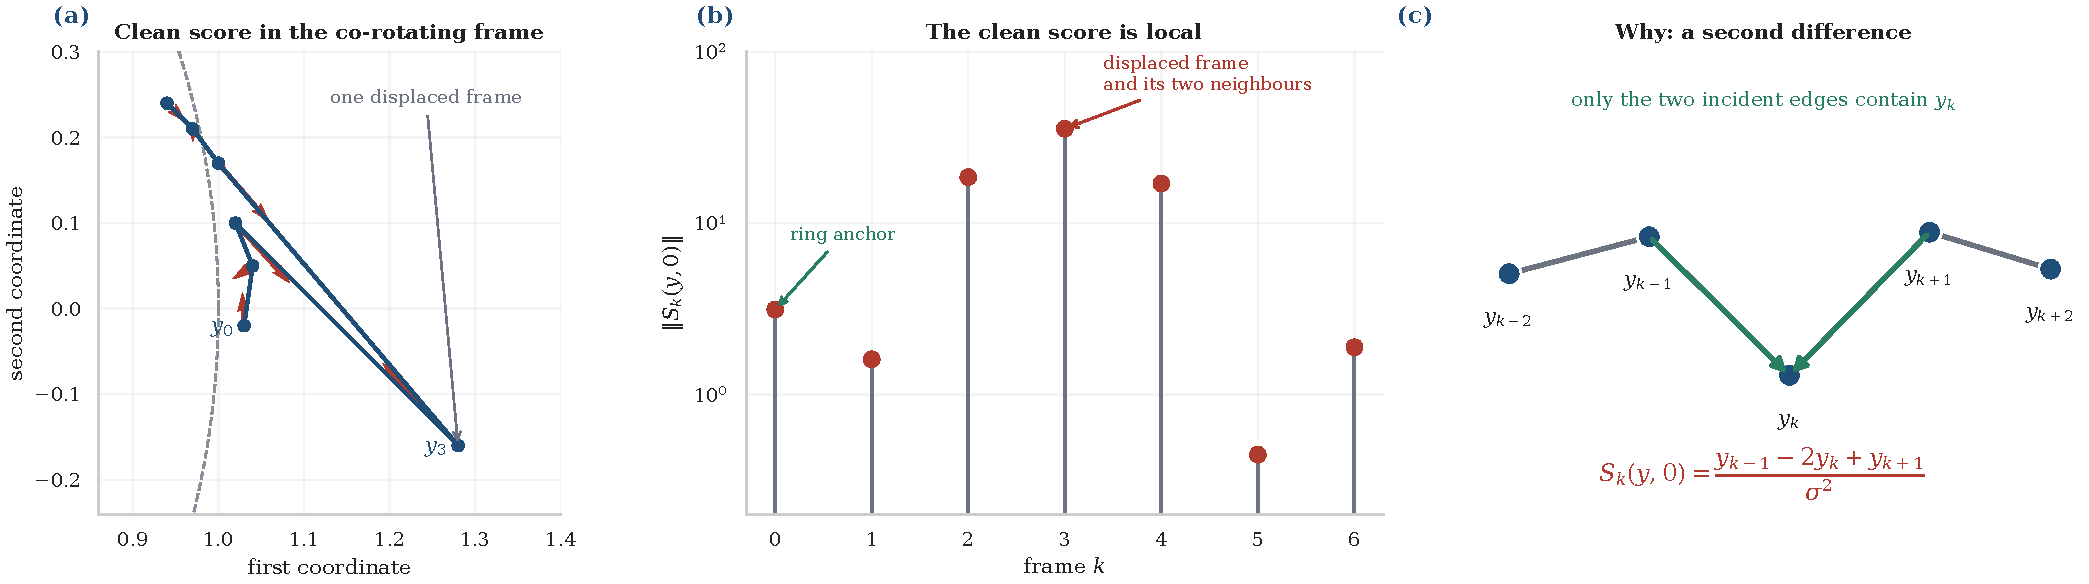
\includegraphics[width=\textwidth]{fig07_clean_score.pdf}
\caption{The clean surrogate score, on a path that co-rotates on the ring except for one
displaced frame ($T=7$, $\sigma=0.15$, $\lambda=0.05$). (a) The score blocks as arrows; lengths
are square-root compressed, since the magnitudes span nearly two decades. (b) The true
magnitudes: only the displaced frame and its two neighbours carry an appreciable score, an
order of magnitude above the rest, and frame $0$ additionally feels the ring anchor.
(c) Why: an interior $y_k$ occurs in exactly two summands of
\eqref{eq:surrogate-logdensity}, one per incident edge, and the two derivatives
\eqref{eq:edge-in}--\eqref{eq:edge-out} combine into a second difference. This locality does
\emph{not} survive noising, as \cref{sec:surrogate-exact} shows.}
\label{fig:clean-surrogate-score}
\end{figure}

\subsection{The noised law, in Kronecker notation}\label{sec:kronecker}

Condition on the anchor. From \eqref{eq:rw-anchor} the frames are Gaussian with
\begin{equation}
 \E[Y_i\given A=a]=a,
 \qquad
 \Cov(Y_i,Y_j\given A=a)
 =\sigma^2\,\E\Big[\Big(\sum_{r\le i}\widetilde\eta_r\Big)
                    \Big(\sum_{s\le j}\widetilde\eta_s\Big)\!\T\Big]
 =\sigma^2\min(i,j)\,I_2 ,
 \label{eq:K-derivation}
\end{equation}
because $\E[\widetilde\eta_r\widetilde\eta_s\T]=\delta_{rs}I_2$, so only the
$\min(i,j)$ indices common to both sums survive. Compactly,

\begin{equation}
 Y\given A=a\ \sim\ \N\big(\mathbf1\otimes a,\;K\otimes I_2\big),
 \qquad K_{ij}=\sigma^2\min(i,j),\quad i,j=0,\ldots,T-1 .
 \label{eq:surrogate-K}
\end{equation}

\begin{definitionbox}[Reading \eqref{eq:surrogate-K}]
$Y$ is the stacked $2T$-vector $(Y_0\T,\ldots,Y_{T-1}\T)\T$, and $\mathbf1\in\R^T$ is the
all-ones vector. The two Kronecker products separate the \emph{temporal} index from the
\emph{spatial} one.
\begin{itemize}
\item $\mathbf1\otimes a=(a\T,a\T,\ldots,a\T)\T\in\R^{2T}$ repeats the same
      two-dimensional anchor in every frame. This is \eqref{eq:rw-anchor}: all frames have the
      same conditional mean.
\item $K\otimes I_2$ has entries
      $(K\otimes I_2)_{(i,\alpha),(j,\beta)}=K_{ij}\,\delta_{\alpha\beta}
      =\Cov\big(Y_i^{(\alpha)},Y_j^{(\beta)}\given A\big)$.
      So $K$ carries all the temporal correlation, and $I_2$ says that the two spatial
      coordinates are uncorrelated and share the \emph{same} temporal covariance --- a
      consequence of the isotropy of the innovations.
\end{itemize}
For $T=3$, written out with $\sigma^2$ factored out of $K$,
\[
 K=\sigma^2\!\begin{pmatrix}0&0&0\\0&1&1\\0&1&2\end{pmatrix},
 \qquad
 K\otimes I_2=\sigma^2\!
 \begin{pmatrix}
 0&0&0&0&0&0\\
 0&0&0&0&0&0\\
 0&0&1&0&1&0\\
 0&0&0&1&0&1\\
 0&0&1&0&2&0\\
 0&0&0&1&0&2
 \end{pmatrix}.
\]
The zero first row and column say that $Y_0=A$ has no innovation noise of its own: given the
anchor it is known exactly. Each scalar entry of $K$ has become a $2\times2$ diagonal block.
\end{definitionbox}

Now apply the channel. With $X=\mt Y+\sqrt{\Dt}\,\Xi$, $\Xi\sim\N(0,I_{2T})$ independent of
$Y$, and using $I_{2T}=I_T\otimes I_2$ to combine the two covariances,
\begin{equation}
 \mt^2(K\otimes I_2)+\Dt(I_T\otimes I_2)=\big(\mt^2K+\Dt I_T\big)\otimes I_2 ,
\end{equation}
so that
\begin{equation}
 X_t\given A=a\ \sim\ \N\big(\mt\,\mathbf1\otimes a,\;C_t\otimes I_2\big),
 \qquad \boxed{\,C_t=\mt^2K+\Dt I_T\,}.
 \label{eq:surrogate-C}
\end{equation}
The crucial feature is that $C_t$ does \emph{not} depend on $a$: the noised law is a
two-parameter \emph{location} mixture of one fixed Gaussian.

\subsection{The anchor posterior is two-dimensional}\label{sec:anchor-posterior}

Define
\begin{equation}
 q=C_t^{-1}\mathbf1\in\R^T,
 \qquad
 \beta=\mt^2\,\mathbf1\T C_t^{-1}\mathbf1\in\R,
 \qquad
 h=\mt\sum_{j=0}^{T-1}q_j\,x_j\in\R^2 .
 \label{eq:q-beta-h}
\end{equation}
Expanding the exponent of \eqref{eq:surrogate-C} in powers of $a$, exactly as in Step~1 of
\cref{tb:response} but now with the correlated covariance $C_t\otimes I_2$, gives
\begin{equation}
 p(a\given x)\propto
 \exp\Big[-\frac{(\|a\|-1)^2}{2\lambda}-\frac{\beta}{2}\|a\|^2+h\T a\Big] .
 \label{eq:anchor-posterior}
\end{equation}
The $2T$-dimensional integral over clean trajectories has collapsed to a
\emph{two-dimensional} posterior over the shared anchor. That is the entire simplification,
and it is a direct consequence of \eqref{eq:rw-anchor}: conditionally on $A$ everything else
is Gaussian and can be integrated out in closed form.

Two moments of \eqref{eq:anchor-posterior} are needed, $\E[A\given x]$ and
$\Cov(A\given x)$. Both are cheap. The prior and the $\|a\|^2$ term are rotationally
symmetric, so the posterior depends on the direction of $a$ only through $h\T a$; therefore
\begin{equation}
 \E[A\given x]=\mu(\rho)\,\ohat h,
 \qquad
 \Cov(A\given x)=v_\perp I_2+(v_\parallel-v_\perp)\,\ohat h\ohat h\T,
 \qquad \rho=\|h\|,\ \ohat h=h/\rho ,
 \label{eq:anchor-moments}
\end{equation}
with three scalar functions of the single scalar $\rho$. They are tabulated once per
$(t,\text{index set})$ by one-dimensional quadrature and interpolated.\footnote{Doing the
angular integral analytically produces modified Bessel functions; \cref{app:anchor} records
the resulting one-dimensional integrals for reproducibility. Nothing in the argument depends
on them --- the posterior is two-dimensional, so any quadrature will do --- and they are not
used again in the main text.}

\subsection{Exact score and exact response}\label{sec:surrogate-exact}

Write $\log p_t(x)=\text{const}-\tfrac12x\T(C_t^{-1}\otimes I_2)x+\log Z(h(x))$, with $Z$ the
normalisation of \eqref{eq:anchor-posterior}. The gradient of the first term is
$-(C_t^{-1}x)_k$ in block $k$; for the second, $\partial h/\partial x_k=\mt q_kI_2$ and
$\nabla_h\log Z=\E[A\given x]$ by \eqref{eq:first-cumulant}. Hence

\begin{keyresult}[Exact surrogate score]
\begin{equation}
 \boxed{\;S_k(x,t)=-\big(C_t^{-1}x\big)_k+\mt\,q_k\,\E[A\given x].}
 \label{eq:surrogate-score}
\end{equation}
\end{keyresult}

The first term is the noised random-walk contribution, near-diagonal in $k$; the second is a
global correction carried by the one shared anchor. Differentiating once more, with
$\partial_{x_j}\E[A\given x]=\mt q_j\Cov(A\given x)$ from \eqref{eq:mean-response-h},

\begin{keyresult}[Exact surrogate response]
\begin{equation}
 \boxed{\;J_{kj}(x,t)=-\big(C_t^{-1}\big)_{kj}I_2+\mt^2\,q_kq_j\,\Cov(A\given x).}
 \label{eq:surrogate-jac}
\end{equation}
\end{keyresult}

The temporal coefficient of the second term is the outer product $qq\T$, which is
\textbf{rank one}. This makes the origin of the long-range part of the response completely
explicit: it is not a chain of local couplings but a single shared latent variable seen by
every frame. \Cref{fig:surrogate-decomposition} separates the two terms.

\begin{figure}[H]
\centering
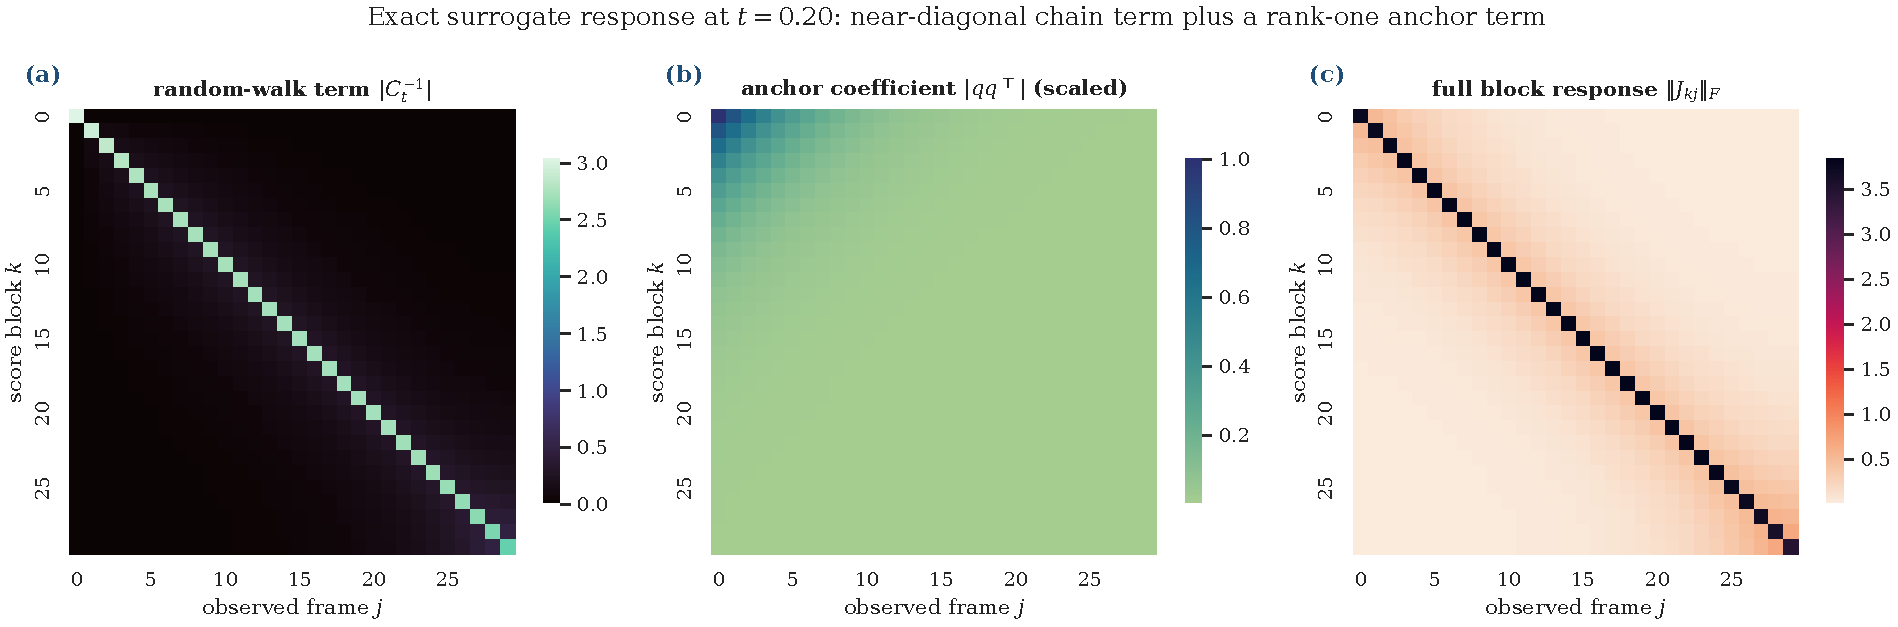
\includegraphics[width=\textwidth]{fig08_surrogate_response.pdf}
\caption{Exact decomposition of the surrogate response at $t=0.20$, $T=30$. (a) The
random-walk term $|C_t^{-1}|$ is concentrated near the diagonal. (b) The anchor coefficient
$|qq\T|$ is rank one and spread over all lags. (c) The average norm of the complete
$2\times2$ blocks. The analytic Jacobian agrees with central finite differences to
$9.2\times10^{-6}$ (\cref{tab:validation}).}
\label{fig:surrogate-decomposition}
\end{figure}

\begin{keyresult}[What the surrogate settles]
Clean Markov locality does not survive marginalisation through the OU channel as locality of
the noised score: \eqref{eq:surrogate-jac} has nonzero blocks at every lag for every $t>0$.
But the nonlocal part is not arbitrary. It decomposes exactly into a near-diagonal chain term
and a rank-one correction generated by the shared ring anchor.
\end{keyresult}

\section{What the surrogate measures}\label{sec:surrogate-measurements}

\paragraph{Protocol.} $T=30$, $\lambda=0.05$, $\sigma=0.15$, $\psi=2\pi/30$; $350$ clean
trajectories, corrupted independently at each diffusion time; anchor moments on $180$
quadrature nodes and a $600$-point interpolation grid in $\|h\|$. In this part the response
profile \eqref{eq:response-profile} is averaged over \emph{all} frame pairs at equal lag rather
than around one central frame, so $L_{\max}=T-1=29$ and the structureless ceilings are
$\bar\ell=15$ and $\xi^{\mathrm{norm}}=29$. The window error \eqref{eq:window-error} is
measured at the central frame $k=15$.

\begin{table}[H]
\centering
\caption{Surrogate diagnostics. ``Marginal RMSE'' is the relative RMS error of replacing the
joint score by per-frame marginal scores. $L_{5\%}$ is the window radius of
\eqref{eq:window-error}. The last row is the value a completely flat profile would give.}
\label{tab:surrogate}
\begin{tabular}{@{}rrrrrrr@{}}
\toprule
$t$ & marginal RMSE & $I_{\rm off}$ & $\bar\ell$ & $\xi^{\rm norm}$ & $\widetilde\Xi$ & $L_{5\%}$ \\
\midrule
0.05 & 0.959 & 6.093 & 2.73 & 2.73 & 1.467 & 6 \\
0.20 & 0.779 & 2.177 & 5.34 & 5.32 & 3.067 & 10 \\
0.70 & 0.462 & 1.171 & 10.61 & 12.61 & 6.994 & 13 \\
1.50 & 0.154 & 0.703 & 13.30 & 20.68 & 6.430 & 11 \\
\midrule
\emph{flat profile} & --- & --- & 15.00 & 29.00 & --- & --- \\
\bottomrule
\end{tabular}

\end{table}

\begin{figure}[H]
\centering
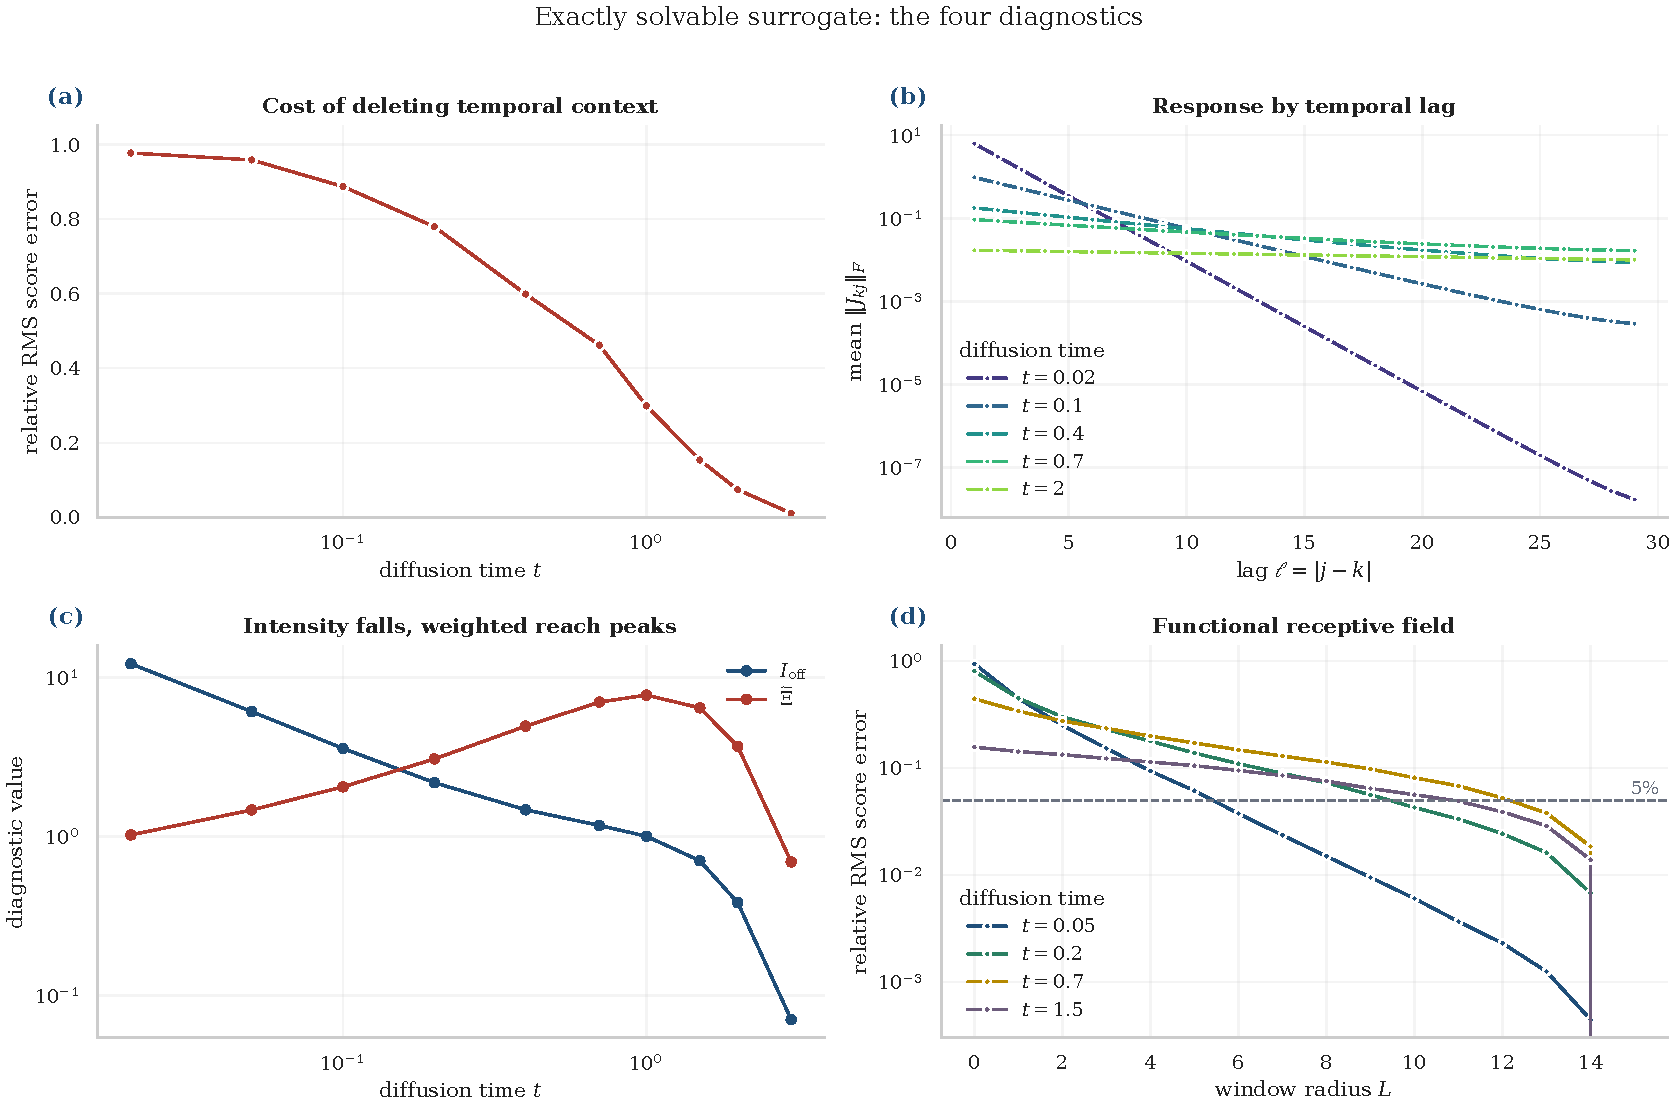
\includegraphics[width=\textwidth]{fig09_surrogate_diagnostics.pdf}
\caption{The exactly solvable surrogate. (a) Relative RMS error from deleting all temporal
context. (b) Response profiles by lag. (c) Intensity falls monotonically while the weighted
reach $\widetilde\Xi$ rises, peaks near $t=1$, and falls again. (d) Window error against
window radius; the dashed line is $5\%$.}
\label{fig:surrogate-summary}
\end{figure}

Three readings.

\textbf{The cost of dropping context is largest at low noise.} At $t=0.02$ the per-frame
marginal score has a relative RMS error of $0.977$ --- it is almost entirely wrong. The error
falls to $0.154$ at $t=1.5$ and $0.011$ at $t=3$. The decline does not mean the joint
structure was unimportant at small $t$; it means that at large $t$ the score itself is
approaching the universal Gaussian field $-x$, which the marginal model also reproduces.

\textbf{Reach and intensity move oppositely.} The intensity $I_{\mathrm{off}}$ falls by a
factor of $173$ between $t=0.02$ and $t=3$, while the weighted mean lag rises from $1.94$ to
$13.9$ frames --- that is, from a genuinely local profile to one close to flat, the
structureless ceiling being $15$. The composite $\widetilde\Xi$ resolves the two: it rises to
$7.7$ at $t=1$ and then falls, which is the behaviour one wants from a single summary.

\textbf{The receptive field is non-monotone.} For a $5\%$ criterion the required window radius
is $L=6,10,13,11$ at $t=0.05,0.20,0.70,1.50$. Context becomes more spread out at intermediate
noise, and then stops mattering at all: the peak of $L_{5\%}$ at $t=0.7$ sits close to the
peak of $\widetilde\Xi$, and neither is captured by $\xi^{\mathrm{norm}}$, which increases
monotonically over the whole range.

\begin{caution}[Scope of Part~I]
This is one parameter set of a model whose later frames are not radially confined. The
qualitative mechanism it exposes --- local clean score, nonlocal noised score, weak but broad
at high noise --- should be checked against the process that was actually drawn on the board.
That is Part~II.
\end{caution}

\FloatBarrier

% ============================================================================
\clearpage
\part{The board problem}
% ============================================================================

\section{The polar process}\label{sec:polar}

\subsection{Polar coordinates, and what we are trying to do}\label{sec:polar-coords}

The board model is naturally written in polar coordinates, so we fix them first. A point
$A\in\R^2$ is described by its distance from the origin and the angle it makes with the first
axis,
\begin{equation}
 A=r\,(\cos\theta,\sin\theta),
 \qquad r=\|A\|\ge0,\qquad \theta\in[0,2\pi) ,
 \label{eq:polar-def}
\end{equation}
and at each point the plane carries a natural moving orthonormal frame,
\begin{equation}
 e_r=(\cos\theta,\sin\theta)
 \quad\text{(radial, pointing away from the origin)},
 \qquad
 e_\theta=(-\sin\theta,\cos\theta)
 \quad\text{(tangential)} .
 \label{eq:moving-frame}
\end{equation}
$e_\theta$ is $e_r$ rotated by a quarter turn, $e_\theta=R_{\pi/2}e_r$, so
$\{e_r,e_\theta\}$ is orthonormal at every $\theta$. Two facts are used repeatedly: moving
along $e_r$ changes the radius at fixed angle, moving along $e_\theta$ changes the angle at
fixed radius; and the area element is $\dd x\dd y=r\dd r\dd\theta$, which is why a density in
$(r,\theta)$ and a density in $(x,y)$ differ by a factor $r$.

The decomposition matters because the model treats the two directions very differently: the
radius is pulled back towards $1$, while the angle drifts steadily and diffuses freely. The
two channels are therefore expected to carry information over different distances, and one aim
of the experiment is to measure that difference.

\Cref{fig:problem-setup} states the problem in these terms. Panels (a)--(c) are the model:
polar coordinates, the confining potential, one clean trajectory. Panel (d) is the goal: given
the whole \emph{noisy} trajectory, the score block at frame $k$ is a posterior estimate of the
clean frame $A_k$, and we want to know which other frames contribute to it, how strongly, and
from how far.

\begin{figure}[H]
\centering
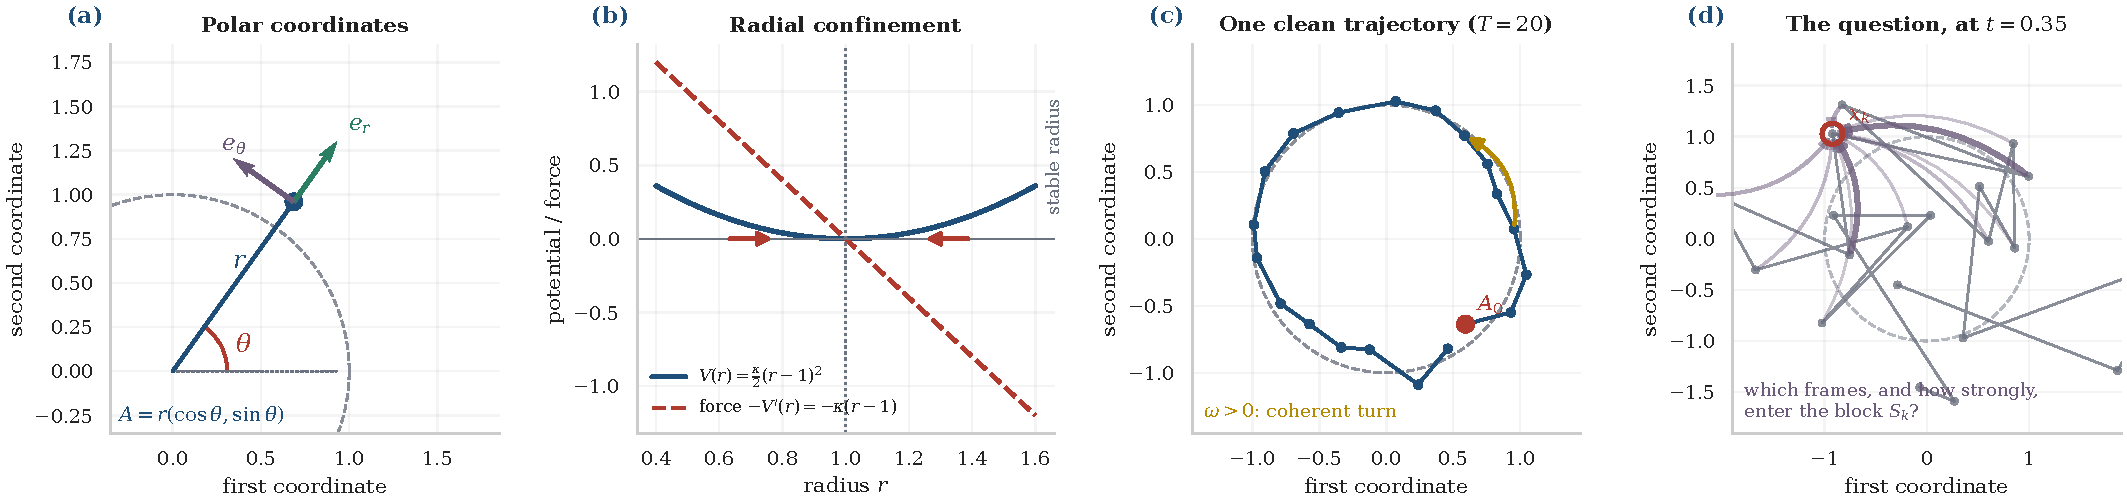
\includegraphics[width=\textwidth]{fig01_problem_setup.pdf}
\caption{The problem. (a) Polar coordinates and the moving frame \eqref{eq:moving-frame}.
(b) The quadratic potential $V(r)=\tfrac{\kappa}{2}(r-1)^2$ and the force $-V'(r)$ it
generates; the force changes sign at $r=1$, which is therefore the stable radius. (c) One
clean trajectory of \eqref{eq:radial-sde}--\eqref{eq:polar-to-cart} at the baseline
parameters: a noisy, coherently turning path near the unit circle. (d) The same trajectory
after the channel \eqref{eq:ou-channel} at $t=0.35$. The score block $S_k$ at the circled
frame is a posterior estimate of the clean $A_k$ built from \emph{all} the noisy frames;
arrow widths indicate the question, not the answer.}
\label{fig:problem-setup}
\end{figure}

\subsection{The equations}

The clean dynamics run in internal time $u$:
\begin{align}
 \dd R_u&=-\kappa(R_u-1)\dd u+\sqrt{2D_r}\dd B_u^{(r)},
 \label{eq:radial-sde}\\
 \dd\Theta_u&=\omega\dd u+\sqrt{2D_\theta}\dd B_u^{(\theta)},
 \label{eq:angular-sde}\\
 A_u&=R_u\,(\cos\Theta_u,\sin\Theta_u),
 \label{eq:polar-to-cart}
\end{align}
with independent Brownian motions. We take the simplest constant-angular-drift reading of the
board; \cref{sec:limitations} records the alternatives.

\subsection{Why the radial drift has this form}

\Cref{eq:radial-sde} is the overdamped Langevin equation \eqref{eq:langevin-overdamped} for the
quadratic potential
\begin{equation}
 V(r)=\frac{\kappa}{2}(r-1)^2 .
 \label{eq:radial-potential}
\end{equation}
A potential is a stored energy, and the force it generates is minus its slope,
\begin{equation}
 F(r)=-V'(r)=-\kappa(r-1) .
 \label{eq:force}
\end{equation}
The minus sign is the whole content: a system pushed by $-V'$ moves \emph{downhill} in $V$,
because then $\tfrac{\dd}{\dd u}V(r_u)=V'(r)\dot r=-V'(r)^2\le0$. Reading off the two cases in
\eqref{eq:force}: if $r>1$ then $F<0$ and the force points inward; if $r<1$ then $F>0$ and it
points outward. The radius is driven towards $1$ from either side, at a rate proportional to
the displacement, with $\kappa$ setting the stiffness. \Cref{fig:problem-setup}(b) draws both
curves. Balancing this force against the noise gives the stationary radial law
$\N(1,D_r/\kappa)$, by \eqref{eq:boltzmann} with $V$ from \eqref{eq:radial-potential} and
$k_BT\mapsto D_r$.

\subsection{Exact radial transition}\label{sec:radial-transition}

We need the law of $R_{k+1}$ given $R_k$ over one internal-time step $h$. Because
\eqref{eq:radial-sde} is linear, this can be obtained exactly, by the same integrating-factor
argument as \cref{tb:ou-channel}.

\begin{toolbox}{The exact one-step radial law}\label{tb:radial}
\textbf{Step 1: shift to the equilibrium radius.} Put $Y_u=R_u-1$. Since $1$ is a constant,
$\dd Y_u=\dd R_u$, and \eqref{eq:radial-sde} becomes a plain OU equation with no offset:
\begin{equation}
 \dd Y_u=-\kappa Y_u\dd u+\sqrt{2D_r}\dd B_u .
 \label{eq:shifted-radial}
\end{equation}

\textbf{Step 2: multiply by the integrating factor $\e^{\kappa u}$.} Consider
$\phi(y,u)=\e^{\kappa u}y$. This is linear in $y$, so $\partial_y^2\phi=0$ and by
\eqref{eq:product-rule} It\^o's lemma reduces to the ordinary product rule --- there is no
correction term:
\begin{align}
 \dd\big(\e^{\kappa u}Y_u\big)
 &=\underbrace{\kappa\e^{\kappa u}Y_u\dd u}_{\partial_u\phi\dd u}
  +\underbrace{\e^{\kappa u}\dd Y_u}_{\partial_y\phi\dd Y}
 \label{eq:radial-product}\\
 &=\kappa\e^{\kappa u}Y_u\dd u
  +\e^{\kappa u}\big(-\kappa Y_u\dd u+\sqrt{2D_r}\dd B_u\big)
 \notag\\
 &=\sqrt{2D_r}\,\e^{\kappa u}\dd B_u .
 \label{eq:radial-exact-differential}
\end{align}
The two drift terms cancel by construction: that is what the factor $\e^{\kappa u}$ is chosen
for. What remains is an exact differential whose right-hand side contains no $Y$, so it can be
integrated directly.

\textbf{Step 3: integrate over one step.} Integrate \eqref{eq:radial-exact-differential} from
$u_k$ to $u_{k+1}=u_k+h$. The left side telescopes:
\begin{equation}
 \e^{\kappa u_{k+1}}Y_{k+1}-\e^{\kappa u_k}Y_k
 =\sqrt{2D_r}\int_{u_k}^{u_{k+1}}\e^{\kappa s}\dd B_s .
\end{equation}
Multiply throughout by $\e^{-\kappa u_{k+1}}$. On the left,
$\e^{-\kappa u_{k+1}}\e^{\kappa u_k}=\e^{-\kappa(u_{k+1}-u_k)}=\e^{-\kappa h}$; on the right,
$\e^{-\kappa u_{k+1}}$ is a constant with respect to the integration variable $s$ and may be
carried inside the integral:
\begin{equation}
 \boxed{\;Y_{k+1}=\e^{-\kappa h}Y_k
 +\sqrt{2D_r}\int_{u_k}^{u_{k+1}}\e^{-\kappa(u_{k+1}-s)}\dd B_s\;.}
 \label{eq:radial-solution}
\end{equation}
The first term is deterministic given $Y_k$; the second is a stochastic integral of a
\emph{deterministic} kernel that weights the noise injected at time $s$ by how much of it has
survived by $u_{k+1}$.

\textbf{Step 4: the stochastic integral has mean zero.} This is \eqref{eq:ito-mean} of
\cref{tb:ito-integral}. In the defining sum, each term is
$f(s_i)\,(B_{s_{i+1}}-B_{s_i})$ with $f(s)=\e^{-\kappa(u_{k+1}-s)}$ a fixed number and the
increment independent of everything up to $s_i$ with mean zero, so every term has mean zero
and so does the limit. Consequently $\E[Y_{k+1}\given Y_k]=\e^{-\kappa h}Y_k$: the conditional
mean simply relaxes geometrically towards $0$, i.e.\ $R$ relaxes towards $1$.

\textbf{Step 5: its variance, by It\^o isometry.} Apply \eqref{eq:ito-isometry} with the same
deterministic $f$, then substitute $v=u_{k+1}-s$, so $\dd v=-\dd s$ and the limits
$s=u_k,u_{k+1}$ become $v=h,0$:
\begin{equation}
 \Var
 =2D_r\int_{u_k}^{u_{k+1}}\e^{-2\kappa(u_{k+1}-s)}\dd s
 =2D_r\int_0^h\e^{-2\kappa v}\dd v
 =2D_r\cdot\frac{1-\e^{-2\kappa h}}{2\kappa}
 =\frac{D_r}{\kappa}\big(1-\e^{-2\kappa h}\big).
 \label{eq:radial-variance}
\end{equation}
Since the kernel is deterministic, the integral is moreover exactly Gaussian
(\cref{tb:ito-integral}).

\textbf{Step 6: name the constants and undo the shift.} Set
\begin{equation}
 a=\e^{-\kappa h},
 \qquad
 q_r=\frac{D_r}{\kappa}\big(1-a^2\big),
 \label{eq:a-qr}
\end{equation}
and return to $R=1+Y$:
\begin{equation}
 \boxed{\;R_{k+1}\given R_k=r\ \sim\ \N\big(1+a(r-1),\,q_r\big).}
 \label{eq:radial-transition}
\end{equation}
\hfill$\square$

\textbf{Two checks.} Because $a\in(0,1)$, the conditional mean $1+a(r-1)$ lies strictly between
$r$ and $1$: one step moves part of the way home. And iterating
\eqref{eq:radial-transition} gives stationary variance $q_r/(1-a^2)=D_r/\kappa$, which is the
Boltzmann value \eqref{eq:boltzmann} for the potential \eqref{eq:radial-potential} --- the
sampled chain and the continuous process agree.
\end{toolbox}

\subsection{Exact angular transition}\label{sec:angular-transition}

\begin{toolbox}{The exact one-step angular law, and why it wraps}\label{tb:angular}
\textbf{Step 1: integrate directly.} The drift in \eqref{eq:angular-sde} does not depend on
$\Theta$, so no integrating factor is needed. Integrating both sides over
$[u_k,u_{k+1}]$ term by term,
\begin{equation}
 \Theta_{k+1}-\Theta_k
 =\int_{u_k}^{u_{k+1}}\!\!\omega\dd u
 +\sqrt{2D_\theta}\int_{u_k}^{u_{k+1}}\!\!\dd B_u^{(\theta)}
 =\omega h+\sqrt{2D_\theta}\,\big(B^{(\theta)}_{u_{k+1}}-B^{(\theta)}_{u_k}\big).
 \label{eq:angular-integrated}
\end{equation}
The first integral is elementary. The second is a stochastic integral with integrand $1$, and
by \eqref{eq:ito-def} it collapses to the single increment
$B_{u_{k+1}}-B_{u_k}$, because every partial sum telescopes.

\textbf{Step 2: the increment.} By the definition of Brownian motion an increment over an
interval of length $h$ is $\N(0,h)$, independent of the past. Multiplying by the constant
$\sqrt{2D_\theta}$ multiplies the variance by $2D_\theta$, so on the real line
\begin{equation}
 \Theta_{k+1}\given\Theta_k=\theta\ \sim\ \N\big(\theta+\omega h,\;q_\theta\big),
 \qquad q_\theta=2D_\theta h .
 \label{eq:angular-line}
\end{equation}
(The It\^o isometry gives the same variance: $2D_\theta\int_{u_k}^{u_{k+1}}1^2\dd s=2D_\theta h$.)

\textbf{Step 3: wrap.} What is observed is the point $A_u=R_u(\cos\Theta_u,\sin\Theta_u)$,
which depends on $\Theta_u$ only modulo $2\pi$. Reducing \eqref{eq:angular-line} modulo $2\pi$
and collecting all the windings that map to the same observed angle,
\[
 \Pr\big[\Theta_{k+1}\bmod2\pi\in\dd\theta'\big]
 =\sum_{n\in\mathbb Z}\Pr\big[\Theta_{k+1}\in\dd\theta'+2\pi n\big],
\]
gives the \emph{wrapped normal} law
\begin{equation}
 \boxed{\;\Theta_{k+1}\given\Theta_k=\theta\ \sim\ \WN\big(\theta+\omega h,\,q_\theta\big),}
 \qquad
 M_\theta(\theta'\given\theta)
 =\sum_{n\in\mathbb Z}\frac{1}{\sqrt{2\pi q_\theta}}
 \exp\Big[-\frac{(\theta'-\theta-\omega h+2\pi n)^2}{2q_\theta}\Big].
 \label{eq:angular-transition}
\end{equation}
When $q_\theta\ll(2\pi)^2$ a single winding dominates and the wrapped normal is
indistinguishable from \eqref{eq:angular-line}; the sum matters only when the angular
uncertainty becomes comparable to a full turn. \hfill$\square$
\end{toolbox}

\begin{figure}[H]
\centering
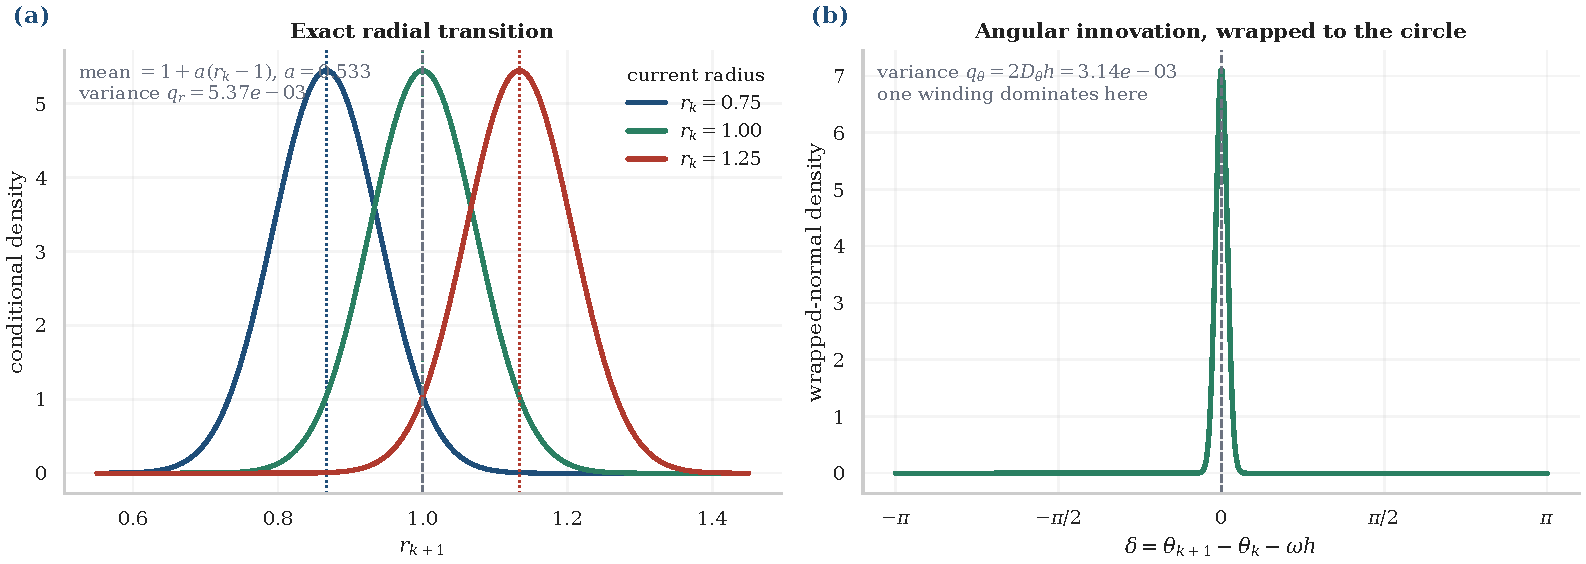
\includegraphics[width=0.9\textwidth]{fig10_transition_kernels.pdf}
\caption{The two one-step transition laws at the baseline parameters. (a) Different current
radii are pulled towards $1$; dotted lines are the conditional means
$1+a(r_k-1)$ of \eqref{eq:radial-transition}. (b) The angular innovation
\eqref{eq:angular-transition}. Since $q_\theta=3.1\times10^{-3}$ is far below $(2\pi)^2$, the
wrapping is invisible here and the turn is sharply concentrated on $\omega h$.}
\label{fig:transition-kernels}
\end{figure}

\subsection{The clean law is Markov, and its score is local}

With $H_k=(R_k,\Theta_k)$ the clean latent law factorises over one-step kernels,
\begin{equation}
 p_0(h_{0:T-1})=p_{\mathrm{init}}(h_0)
 \prod_{k=0}^{T-2}M_r(r_{k+1}\given r_k)\,M_\theta(\theta_{k+1}\given\theta_k) ,
 \label{eq:polar-joint}
\end{equation}
with $M_r$ from \eqref{eq:radial-transition} and $M_\theta$ from
\eqref{eq:angular-transition}. This is the precise sense in which the clean trajectory is
Markov, and it is the structure the research question asks us to exploit. We initialise at the
stationary radial law $R_0\sim\N(1,D_r/\kappa)$ and a uniform phase
$\Theta_0\sim\mathrm{Unif}[0,2\pi)$.

Differentiating \eqref{eq:polar-joint} gives a local clean score, by the same two-incident-edges
counting as in \cref{sec:surrogate-score}. With the radial innovation
$\varepsilon_k^{(r)}=R_{k+1}-1-a(R_k-1)$,
\begin{equation}
 \boxed{\;\frac{\partial}{\partial R_k}\log p_0
 =-\frac{\varepsilon_{k-1}^{(r)}}{q_r}+a\,\frac{\varepsilon_k^{(r)}}{q_r}\;}
 \label{eq:clean-radial-score}
\end{equation}
for an interior frame: the first term checks consistency with where the previous radius left
off, the second checks the prediction for the next. For the angle, with the wrapped innovation
$\delta_k=\wrap(\Theta_{k+1}-\Theta_k-\omega h)$ and
$s_q(\delta)=\frac{\dd}{\dd\delta}\log\sum_n\exp[-(\delta+2\pi n)^2/2q]$
(\cref{app:wrapped}),
\begin{equation}
 \boxed{\;\frac{\partial}{\partial\Theta_k}\log p_0
 =s_{q_\theta}(\delta_{k-1})-s_{q_\theta}(\delta_k)\;.}
 \label{eq:clean-angular-score}
\end{equation}
When one winding dominates, $s_q(\delta)\approx-\delta/q$ and \eqref{eq:clean-angular-score}
becomes the familiar difference of neighbouring angular innovations.

Finally, to compare with the Cartesian score we must change variables. Because
$\dd x\dd y=r\dd r\dd\theta$, the Cartesian density carries an extra factor $1/r$ relative to
the polar one, and projecting the polar gradient onto the moving frame
\eqref{eq:moving-frame} gives
\begin{equation}
 \boxed{\;\nabla_{A_k}\log p_0
 =e_{r,k}\Big(\partial_{r_k}\log p_0-\frac1{r_k}\Big)
 +\frac{e_{\theta,k}}{r_k}\,\partial_{\theta_k}\log p_0\;.}
 \label{eq:polar-cart-score}
\end{equation}
The factor $1/r_k$ on the tangential component is the usual polar metric factor: a given
change of angle moves the point farther when the radius is larger.

This clean score is local in internal time. The next section explains why the noised one is
not.

\section{The noised joint score}\label{sec:polar-noised}

\subsection{Why there is no closed form}

At diffusion time $t$ the channel \eqref{eq:ou-channel} acts on each frame,
\begin{equation}
 X_k\given R_k,\Theta_k\ \sim\
 \N\Big(\mt R_k\big(\cos\Theta_k,\sin\Theta_k\big)\T,\ \Dt I_2\Big)
 \;=:\;g_t(x_k\given h_k) ,
 \label{eq:polar-likelihood}
\end{equation}
and the noised density is the integral over all latent trajectories,
\begin{equation}
 p_t(x)=\int p_{\mathrm{init}}(h_0)
 \prod_{k=0}^{T-2}M(h_{k+1}\given h_k)
 \prod_{k=0}^{T-1}g_t(x_k\given h_k)\dd h_{0:T-1} .
 \label{eq:polar-noised-density}
\end{equation}
The integral has no simple global closed form, because the observation map
\[
 (r,\theta)\mapsto r(\cos\theta,\sin\theta)
\]
is nonlinear and periodic. This is the one structural difference from Part~I. There, the
conditional law given the anchor was Gaussian with an $a$-independent covariance, so the
latent integral collapsed to two dimensions. Here the latent state enters the likelihood
through a nonlinear function, and no such collapse is available.

\subsection{What Markovity buys instead}

The factorisation \eqref{eq:polar-joint} nonetheless makes \eqref{eq:polar-noised-density}
tractable, by replacing one $2T$-dimensional integral with $2T$ two-dimensional ones. Define a
forward function
\begin{align}
 f_0(h_0)&=p_{\mathrm{init}}(h_0)\,g_t(x_0\given h_0),\notag\\
 f_{k+1}(h_{k+1})&=g_t(x_{k+1}\given h_{k+1})
 \int M(h_{k+1}\given h_k)f_k(h_k)\dd h_k ,
 \label{eq:forward-recursion}
\end{align}
and a backward function
\begin{align}
 b_{T-1}(h_{T-1})&=1,\notag\\
 b_k(h_k)&=\int M(h_{k+1}\given h_k)\,g_t(x_{k+1}\given h_{k+1})\,b_{k+1}(h_{k+1})
 \dd h_{k+1} .
 \label{eq:backward-recursion}
\end{align}
The smoothed one-frame posterior is then $p(h_k\given x)\propto f_k(h_k)b_k(h_k)$, and
\begin{equation}
 \E[A_k\given x]=\int r\,(\cos\theta,\sin\theta)\T\,p(r,\theta\given x)\dd r\dd\theta ,
 \label{eq:polar-posterior-mean}
\end{equation}
after which the score follows from \eqref{eq:block-score} and the response from
\eqref{eq:fdt}.

\begin{intuition}[How clean Markovity is exploited]
The noised score can depend on every frame, but distant information cannot jump directly to
frame $k$: it is transmitted through a sequence of one-step transition integrals. Two things
follow. Computationally, the cost is linear in $T$ rather than exponential. Structurally, the
decay of the response with lag is a property of the one-step kernel, which is why the
parameter sweeps of \cref{sec:measurements} can predict it.
\end{intuition}

\paragraph{Numerical representation.} The integrals are evaluated on a polar grid,
$r\in[0.45,1.55]$ with $41$ points and $\theta\in[0,2\pi)$ with $128$ points for the response
study. The radial interval spans more than six stationary standard deviations. Each one-step
kernel is normalised on the grid, and the forward and backward functions are rescaled at every
step to avoid underflow. The resulting score is exact for the discretised latent state space;
\cref{sec:validation} measures the remaining grid error.

\subsection{Looking at the score}

The full score lives in $\R^{2T}$ and cannot be drawn. To see block $S_k$ we fix every noisy
frame except $x_k$ and vary $x_k\in\R^2$; since
$\nabla_{x_k}\log p_t(x_k\given x_{-k})=S_k(x,t)$, this is an exact two-dimensional
conditional slice, not an approximation.

\begin{figure}[H]
\centering
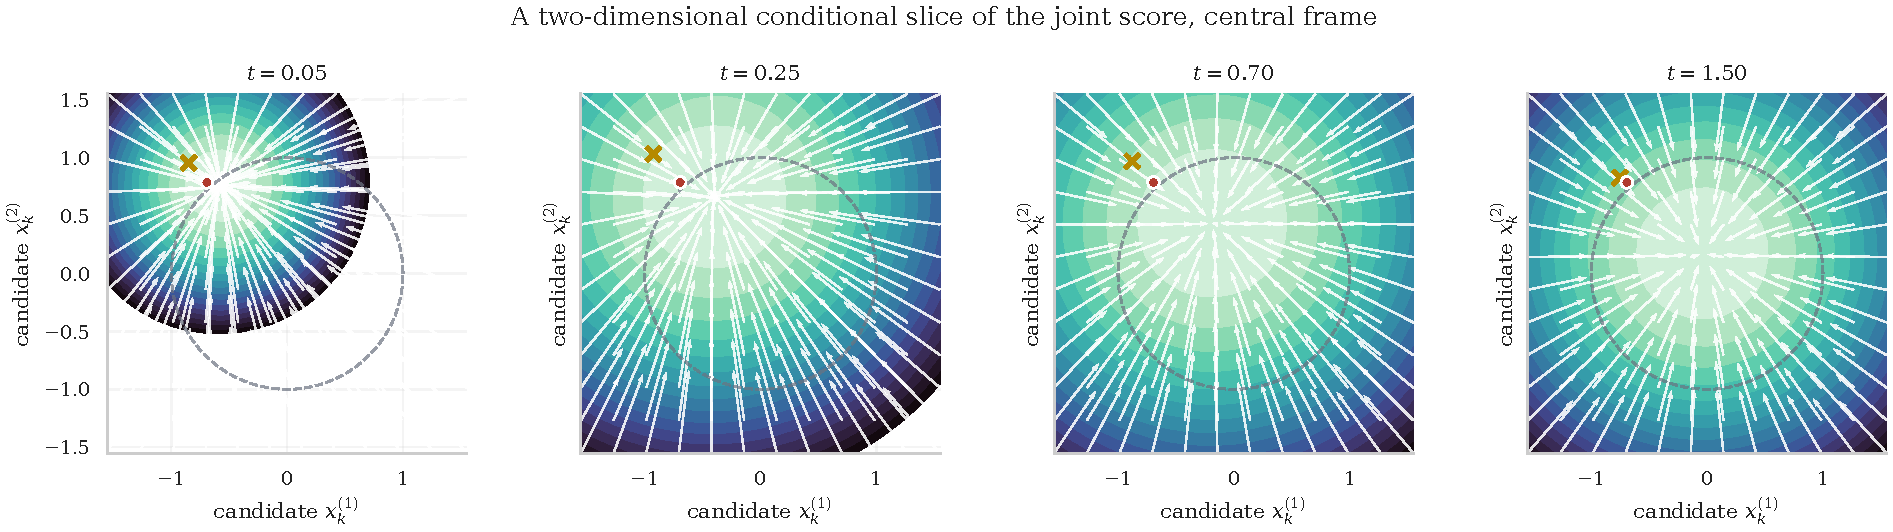
\includegraphics[width=\textwidth]{fig11_joint_score_fields.pdf}
\caption{Conditional slices of the joint score at the central frame. Contours are
$\log p_t(x_k\given x_{-k})$, arrows the score. The red dot is the clean frame, the gold cross
its noisy observation. At small $t$ the other frames identify a specific phase on the ring; as
$t$ grows the field smooths out and approaches the Gaussian field $-x_k$.}
\label{fig:exact-score-fields}
\end{figure}

\begin{figure}[H]
\centering
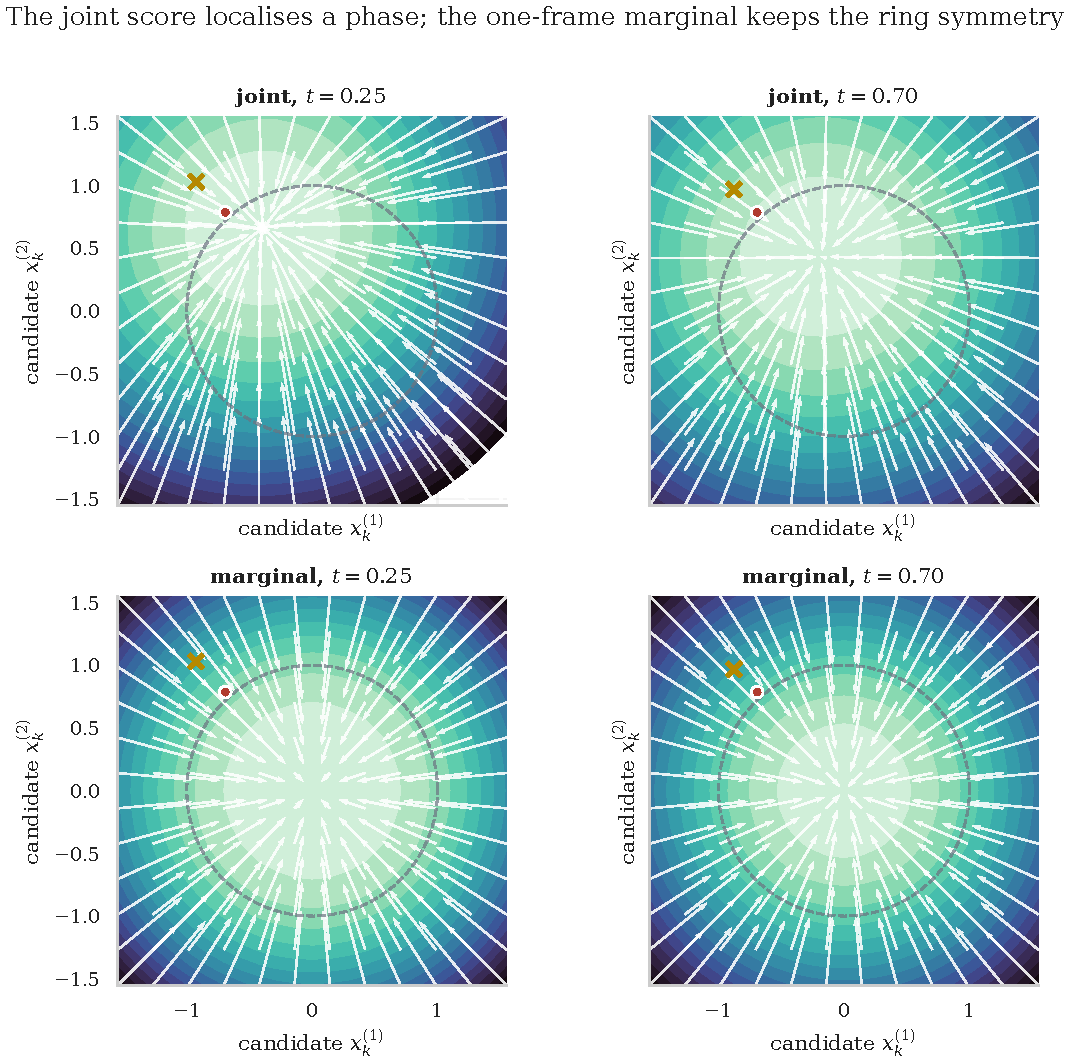
\includegraphics[width=0.72\textwidth]{fig12_joint_vs_marginal_fields.pdf}
\caption{The two objects of \eqref{eq:joint-marg-gap}, drawn. Top: the joint conditional field
is localised near the phase inferred from the rest of the trajectory. Bottom: the one-frame
marginal field stays close to ring-symmetric, because one frame alone does not identify where
along the ring the trajectory is. This is the picture behind \cref{fig:score-graphs}.}
\label{fig:joint-marg-fields}
\end{figure}

\section{A local linear model}\label{sec:taylor}

The grid calculation is exact but opaque. A first-order expansion around a single rotating
branch turns the model into a linear Gaussian state-space model, which can be read
analytically. We derive it, and then state carefully when it may be used.

\subsection{The expansion, order by order}

Take the deterministic reference path $\bar R_k=1$, $\bar\Theta_k=\theta_0+k\omega h$ and write
the deviations as
\begin{equation}
 R_k=1+\rho_k,\qquad \Theta_k=\bar\Theta_k+\varphi_k ,
\end{equation}
with $e_{r,k},e_{\theta,k}$ the moving frame \eqref{eq:moving-frame} evaluated at
$\bar\Theta_k$. Rotating the reference direction by $\varphi_k$,
\begin{equation}
 \big(\cos\Theta_k,\sin\Theta_k\big)
 =\cos\varphi_k\,e_{r,k}+\sin\varphi_k\,e_{\theta,k} ,
\end{equation}
so that, exactly,
\begin{equation}
 A_k=(1+\rho_k)\big(\cos\varphi_k\,e_{r,k}+\sin\varphi_k\,e_{\theta,k}\big).
 \label{eq:taylor-exact}
\end{equation}
Now insert $\cos\varphi=1-\tfrac{\varphi^2}{2}+O(\varphi^4)$ and
$\sin\varphi=\varphi-\tfrac{\varphi^3}{6}+O(\varphi^5)$ and expand:
\begin{equation}
 A_k=\underbrace{e_{r,k}+\rho_k e_{r,k}+\varphi_k e_{\theta,k}}_{\text{first order}}
 \;\underbrace{-\tfrac12\varphi_k^2e_{r,k}+\rho_k\varphi_ke_{\theta,k}}_{\text{second order}}
 \;+\;O\big(\|(\rho_k,\varphi_k)\|^3\big).
 \label{eq:taylor-full}
\end{equation}
Keeping the first order only:

\begin{keyresult}[Local Cartesian linearisation]
\begin{equation}
 \boxed{\;A_k\approx e_{r,k}+\rho_k\,e_{r,k}+\varphi_k\,e_{\theta,k}\;}
 \label{eq:taylor-first}
\end{equation}
\end{keyresult}

Radial deviations move perpendicular to the ring, angular deviations along the tangent, and to
this order the two are decoupled. The two discarded terms have clear meanings: $-\tfrac12
\varphi^2e_r$ is the curvature of the circle, which the tangent plane cannot see, and
$\rho\varphi e_\theta$ is the fact that at larger radius a given angular deviation moves the
point farther.

The truncation error is therefore quadratic. For a pure angular deviation at $\rho=0$,
\begin{equation}
 \big\|A_k-\ohat A_k\big\|
 =\big\|(\cos\varphi-1,\ \sin\varphi-\varphi)\big\|
 =\tfrac{\varphi^2}{2}+O(\varphi^3),
 \label{eq:taylor-error}
\end{equation}
and keeping the second order reduces it to $\varphi^3/6$.
\Cref{fig:taylor}(a,b) shows both.

\subsection{The linear Gaussian model it produces}

Two of the three ingredients are already exactly linear. The radial deviation follows
\eqref{eq:radial-transition} verbatim,
\begin{equation}
 \rho_{k+1}=a\rho_k+\sqrt{q_r}\,\xi_k^{(r)} ,
 \label{eq:rho-ar1}
\end{equation}
an AR(1) chain, and on one unwrapped angular branch \eqref{eq:angular-line} gives a random
walk,
\begin{equation}
 \varphi_{k+1}=\varphi_k+\sqrt{q_\theta}\,\xi_k^{(\theta)} .
 \label{eq:phi-rw}
\end{equation}
Together with the linear observation \eqref{eq:taylor-first} and the linear channel
\eqref{eq:ou-channel}, the whole trajectory is jointly Gaussian, $X_t\approx\N(\mu_t,\Sigma_t)$,
and its score is explicit:

\begin{keyresult}[Taylor score]
\begin{equation}
 \boxed{\;S^{\mathrm{lin}}(x,t)=-\Sigma_t^{-1}(x-\mu_t).}
 \label{eq:linear-score}
\end{equation}
\end{keyresult}

\subsection{When the expansion can hold, and when it cannot}\label{sec:taylor-validity}

\Cref{eq:taylor-error} makes the condition quantitative: the linearisation is accurate while
the angular deviation from the reference branch stays small, and by
\eqref{eq:taylor-error} a $5\%$ error in units of the ring radius corresponds to
$\varphi\approx0.32$~rad. Two different quantities must be checked against that number.

\textbf{The clean spread is small.} The angular deviation of the clean process is the random
walk \eqref{eq:phi-rw}, so after $T-1$ steps its standard deviation is
$\sqrt{q_\theta(T-1)}$. At the baseline, $q_\theta=2D_\theta h=3.14\times10^{-3}$ and $T=20$
give $0.244$~rad. The clean trajectory therefore stays within roughly a quarter of a radian of
a single rotating branch over its whole length, and expanding around one branch is reasonable
\emph{for the prior}.

\textbf{The posterior spread is what actually matters.} The score involves the posterior of
$\Theta_k$ given the noisy trajectory, and that spreads as $t$ grows. Measuring it directly
--- the circular standard deviation of the smoothed angular posterior at the central frame,
averaged over six trajectories --- gives $0.085$~rad at $t=0.03$, $0.25$~rad at $t=0.4$,
$0.40$~rad at $t=0.7$ and $1.62$~rad at $t=2$. The threshold $0.32$~rad is crossed near
$t\approx0.55$, and \cref{fig:taylor}(c) shows the measured score error beginning to grow just
after it.

\begin{caution}[The limits of one tangent plane]
The expansion is local and phase-conditioned. It cannot represent a posterior spread over a
large arc, several wrapped angular branches, or a multimodal phase. Beyond the crossing point
these are not small effects to be bounded but qualitatively absent features, and the honest
procedure is to compare against the nonlinear grid calculation --- which is what
\cref{tab:taylor} does. A second caveat is independent of $t$: the reference phase $\theta_0$
must be estimated from the data, and the resulting error does not vanish as $t\to0$. It is
visible in \cref{tab:taylor} as a floor of $3$--$4\%$ on the central-block error even at the
smallest diffusion times, where the angular spread is negligible.
\end{caution}

\begin{figure}[H]
\centering
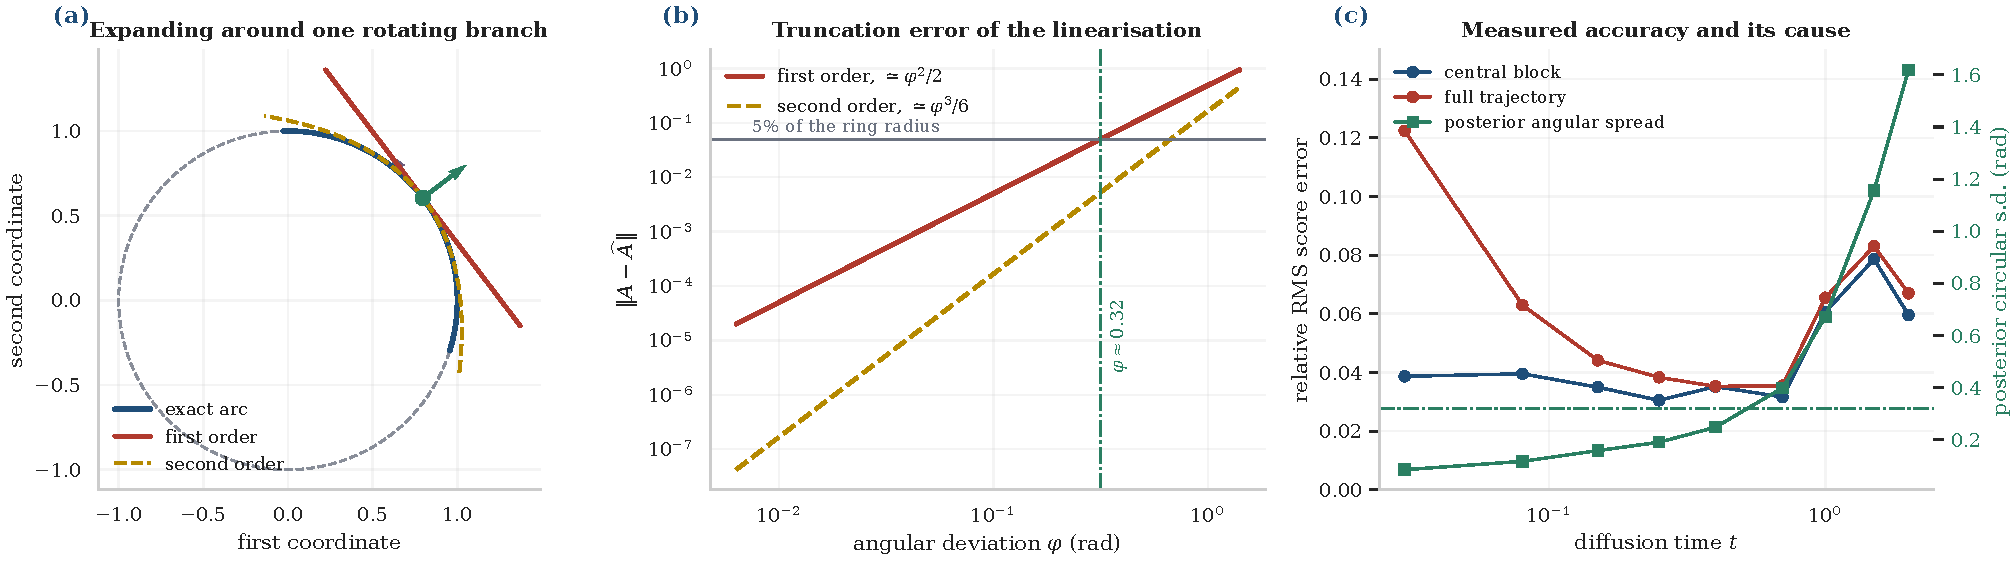
\includegraphics[width=\textwidth]{fig13_taylor.pdf}
\caption{The linearisation and its validity. (a) Exact arc, first-order tangent, and
second-order parabola through the reference point, with the moving frame. (b) Truncation
error against angular deviation: first order is $O(\varphi^2)$ and second order
$O(\varphi^3)$, so a $5\%$ error corresponds to $\varphi\approx0.32$~rad. (c) Measured
relative score error of \eqref{eq:linear-score} against the nonlinear grid score (left axis),
together with the measured circular standard deviation of the smoothed angular posterior
(right axis). The error starts to grow shortly after the posterior spread crosses the
threshold.}
\label{fig:taylor}
\end{figure}

\subsection{Analytic reach in the local model}\label{sec:analytic-reach}

The value of \eqref{eq:linear-score} is that its response can be computed by hand, which turns
the vague statement ``the one-step dynamics control the reach'' into a formula. For an
infinite interior chain, the AR(1) prior \eqref{eq:rho-ar1} has Fourier-space precision
\begin{equation}
 Q_r(\varpi)=\frac{1+a^2-2a\cos\varpi}{q_r} ,
\end{equation}
and the local observation \eqref{eq:polar-likelihood} contributes precision
$\lambda_t=\mt^2/\Dt$ at every frame. The posterior covariance in Fourier space is therefore
$\ohat C_r(\varpi;t)=(\lambda_t+Q_r(\varpi))^{-1}$, and defining $\gamma_r$ by
\begin{equation}
 \cosh\gamma_r=\frac{1+a^2+q_r\lambda_t}{2a} ,
 \label{eq:gamma-r}
\end{equation}
the inverse transform is a pure exponential,
\begin{equation}
 C_r(\ell,t)=\frac{q_r}{2a\sinh\gamma_r}\,\e^{-\gamma_r|\ell|},
 \qquad \xi_r^{\mathrm{lin}}(t)=\gamma_r^{-1} .
 \label{eq:linear-radial-cov}
\end{equation}
The angular channel is the $a\to1$ case,
\begin{equation}
 \cosh\gamma_\theta=1+\frac{q_\theta\lambda_t}{2},
 \qquad
 C_\theta(\ell,t)=\frac{q_\theta}{2\sinh\gamma_\theta}\,\e^{-\gamma_\theta|\ell|} ,
 \label{eq:linear-angular-cov}
\end{equation}
and by the response identity \eqref{eq:fdt} the score responses are
\begin{equation}
 J_r(\ell,t)=\frac{\mt^2}{\Dt^2}C_r(\ell,t),
 \qquad
 J_\theta(\ell,t)=\frac{\mt^2}{\Dt^2}C_\theta(\ell,t) .
 \label{eq:linear-response}
\end{equation}

\Cref{eq:linear-response} separates reach from amplitude explicitly, and in opposite
directions. As $t$ grows, $\lambda_t\to0$, so $\gamma\to0$ and the covariance length
\emph{increases}; at the same time the prefactor $\mt^2/\Dt^2\to0$, so the score response
\emph{vanishes}. This is the mechanism that \cref{sec:weighted-reach} was built to summarise,
now visible in closed form.

\paragraph{Clean correlation scales.} For orientation, the clean process has stationary radial
covariance $\Cov(\rho_k,\rho_{k+\ell})=(D_r/\kappa)\e^{-\kappa h|\ell|}$, hence
$\xi_r^{\mathrm{clean}}=1/(\kappa h)$, and first-harmonic angular coherence
$\E[\e^{i(\Theta_{k+\ell}-\Theta_k)}]=\e^{i\omega h\ell}\e^{-D_\theta h|\ell|}$, hence
$\xi_\theta^{\mathrm{clean}}=1/(D_\theta h)$. At the baseline $h=2\pi/20\approx0.314$, so
\[
 \xi_r^{\mathrm{clean}}\approx1.6\ \text{frames},
 \qquad
 \xi_\theta^{\mathrm{clean}}\approx637\ \text{frames} .
\]
The angular coherence length exceeds the length of the trajectory by more than a factor of $30$: within
one data point the phase is essentially a single coherent quantity, while the radius forgets
itself after a couple of frames. This asymmetry is the prediction that
\cref{sec:measurements} tests.

\section{Measurements}\label{sec:measurements}

\paragraph{Protocol.} $T=20$, $\kappa=2$, $D_r=0.015$, $D_\theta=0.005$, $\omega=1$,
$h=2\pi/20$, so the stationary radial standard deviation is $\sqrt{D_r/\kappa}=0.087$. Per
diffusion time, $28$ independent clean trajectories for the response study and $36$ for the
window study; central frame $k=10$, so $L_{\max}=10$ and the structureless ceilings are
$\bar\ell=5.5$ and $\xi^{\mathrm{norm}}=10$. The radial and tangential projections
\begin{equation}
 J^{rr}_{kj}=e_{r,k}\T J_{kj}e_{r,j},
 \quad
 J^{\theta\theta}_{kj}=e_{\theta,k}\T J_{kj}e_{\theta,j},
 \quad\text{etc.},
 \label{eq:projected-response}
\end{equation}
use the \emph{simulated} clean angle as an oracle basis. That is a diagnostic convenience, not
an ingredient of the score; \cref{sec:limitations} returns to it.

\begin{table}[H]
\centering
\caption{Original polar model: reach and weighted reach by channel, the cost of dropping
context, and the window radii. $\bar\ell$ is the weighted mean lag \eqref{eq:mean-lag},
$\widetilde\Xi$ the relative weighted reach \eqref{eq:weighted-reach}, $L^{5\%}$ the receptive
radius \eqref{eq:window-error}. The structureless ceiling for $\bar\ell$ is $5.5$.}
\label{tab:polar-response}
\begin{tabular}{@{}rrrrrrrr@{}}
\toprule
$t$ & marg.\ RMSE & $\bar\ell_r$ & $\bar\ell_\theta$ & $\widetilde\Xi_r$ & $\widetilde\Xi_\theta$ & $L_r^{5\%}$ & $L_\theta^{5\%}$ \\
\midrule
0.03 & 0.732 & 1.98 & 4.19 & 0.208 & 2.166 & 2 & 9 \\
0.10 & 0.733 & 2.71 & 5.01 & 0.119 & 2.575 & 3 & 9 \\
0.40 & 0.513 & 5.04 & 5.40 & 0.314 & 2.672 & 7 & 9 \\
0.70 & 0.349 & 5.47 & 5.45 & 1.292 & 2.701 & 8 & 9 \\
1.00 & 0.229 & 5.46 & 5.46 & 1.022 & 1.793 & 8 & 9 \\
1.50 & 0.092 & 5.48 & 5.47 & 0.928 & 1.042 & 5 & 7 \\
2.00 & 0.037 & 5.47 & 5.47 & 0.428 & 0.428 & 0 & 0 \\
\bottomrule
\end{tabular}

\end{table}

\subsection{Joint versus marginal}

Replacing the joint score by per-frame marginal scores costs a relative RMS error of $0.73$ at
$t=0.03$. The error stays above $0.69$ up to $t=0.2$, then falls, passing below $0.10$ only
around $t=1.5$. The nonlinear process therefore agrees with the surrogate that the effect is
not an artefact of the Gaussian construction. \Cref{fig:joint-marg-fields} shows the
mechanism: one frame alone does not identify where along the ring the trajectory is.

\subsection{The radial and tangential channels differ}

\begin{figure}[H]
\centering
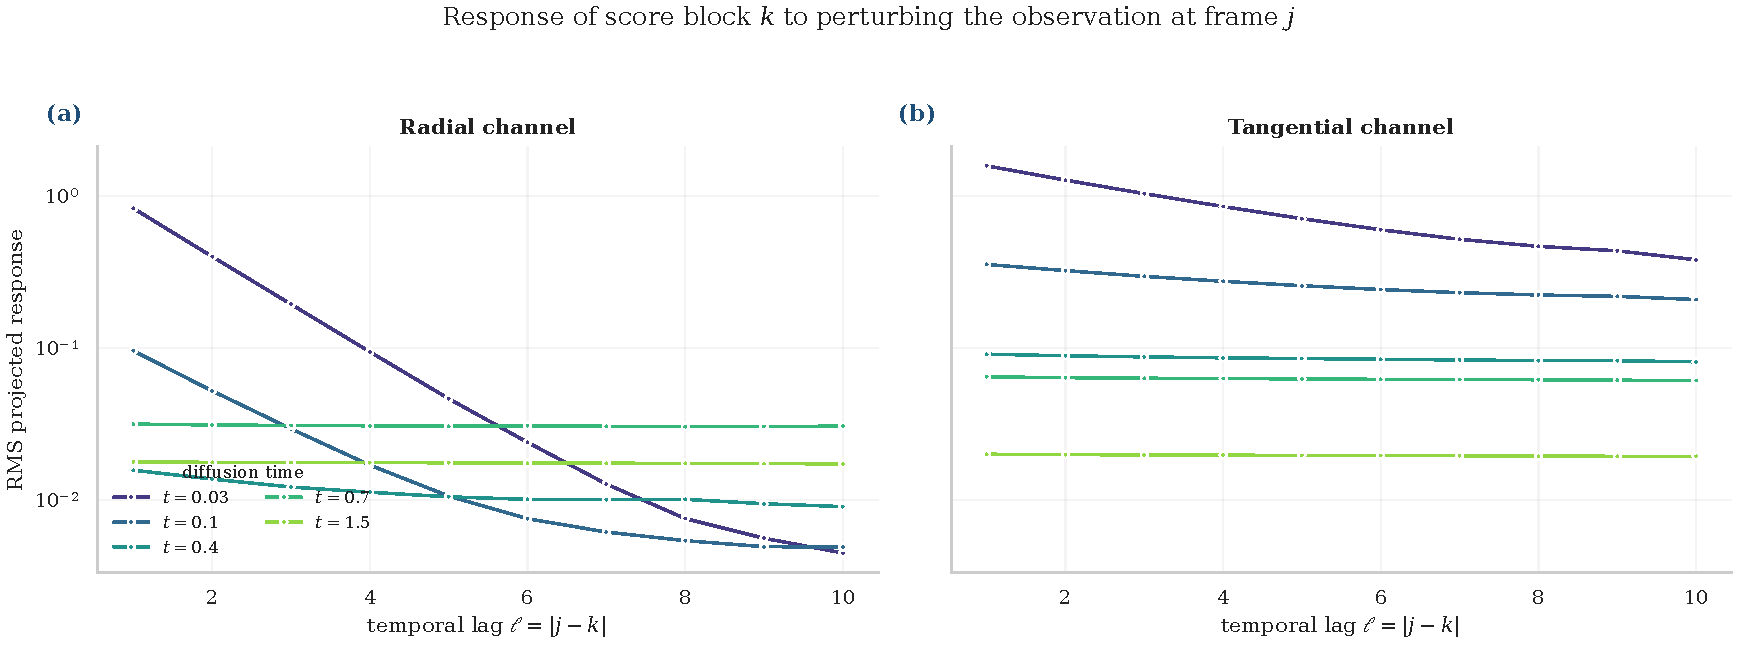
\includegraphics[width=\textwidth]{fig14_response_profiles.pdf}
\caption{Projected response profiles \eqref{eq:projected-response}. At small $t$ the radial
channel decays quickly with lag while the tangential channel is nearly flat across the whole
trajectory. At larger $t$ both profiles flatten, but their absolute levels are an order of
magnitude lower.}
\label{fig:response-profiles}
\end{figure}

At $t=0.03$ the weighted mean lag is $1.98$ frames radially and $4.19$ frames tangentially,
and the gap is much wider once intensity is included: $\widetilde\Xi_r=0.21$ against
$\widetilde\Xi_\theta=2.17$, a factor of ten. The normalised range would have reported the
same contrast as a factor of $2.5$ only. This is the clean-scale prediction of
\cref{sec:analytic-reach} confirmed: radial fluctuations are damped by mean reversion after
$\xi_r^{\mathrm{clean}}\approx1.6$ frames, while the phase is coherent over far more frames
than the trajectory contains.

The local linear model is quantitatively right where it should be. At $t=0.03$ it predicts a
radial e-folding length of $1.35$ frames, against a measured exponential fit of $1.39$ frames
--- agreement to $3\%$ (\cref{tab:exp-fits}). Its tangential prediction, $4.45$ frames, is
already comparable to the chain, and the measured fit of $6.36$ frames should be read as
finite-size dominated rather than as an estimate of an infinite-system length.

\begin{table}[H]
\centering
\caption{Low-noise exponential fits of the response profiles. These are reported for
comparison with the analytic lengths of \cref{sec:analytic-reach}, and only at the three
smallest diffusion times: beyond those the profiles are too flat for the fit to mean
anything, and $\xi_\theta^{\mathrm{exp}}$ exceeds $290$ frames in a chain of $20$. The
bounded diagnostics of \cref{sec:diagnostics} are used everywhere else.}
\label{tab:exp-fits}
\begin{tabular}{@{}rrrrr@{}}
\toprule
$t$ & $\xi_r^{\rm exp}$ & $R_r^2$ & $\xi_\theta^{\rm exp}$ & $R_\theta^2$ \\
\midrule
0.03 & 1.39 & 1.000 & 6.36 & 0.979 \\
0.06 & 1.57 & 0.999 & 11.24 & 0.967 \\
0.10 & 2.99 & 0.901 & 17.37 & 0.963 \\
\bottomrule
\end{tabular}

\end{table}

\subsection{Reach and intensity move in opposite directions}

\begin{figure}[H]
\centering
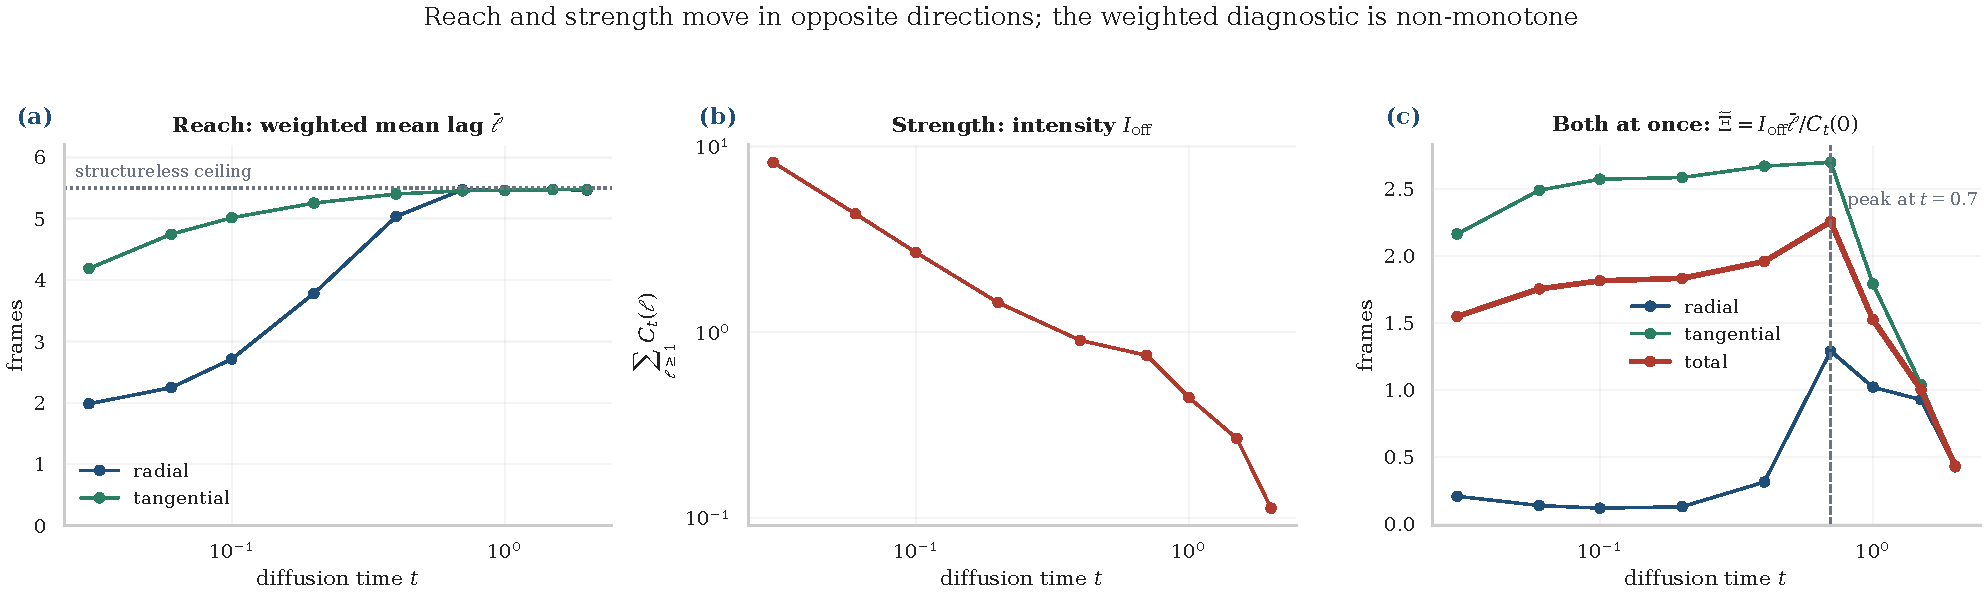
\includegraphics[width=\textwidth]{fig15_range_intensity.pdf}
\caption{Reach, strength, and the two combined. (a) The weighted mean lag rises towards its
structureless ceiling, the radial channel much later than the tangential one. (b) The absolute
cross-frame intensity falls by a factor of about $73$ over the same range. (c) The relative
weighted reach $\widetilde\Xi$ is non-monotone in all three channels, peaking at $t=0.7$.}
\label{fig:range-intensity}
\end{figure}

The two elementary diagnostics disagree, and both are right. Between $t=0.03$ and $t=2$ the
intensity $I_{\mathrm{off}}$ falls from $8.2$ to $0.11$, a factor of about $73$, while the
weighted mean lag rises from $4.10$ to $5.48$ frames --- that is, to within $0.4\%$ of the
structureless ceiling $5.5$. The correct reading is not that high-noise frames are strongly
coupled; it is that the weak residual coupling is spread evenly over the chain.

The composite $\widetilde\Xi$ turns this into one number, and \cref{fig:metric-construction}(c)
is the payoff. $\widetilde\Xi$ rises from $1.55$ at $t=0.03$ to $2.26$ at $t=0.7$ and then
falls to $0.43$ at $t=2$. The independently measured receptive radius $L_{5\%}$ does the same
thing --- $8,8,9,9,9,6,0$ across $t=0.03,\ldots,2$ --- while $\xi^{\mathrm{norm}}$ rises
monotonically over the whole range and reports nothing about the turn. Two remarks, in the
interest of not over-claiming: the peaks do not coincide exactly (the surrogate has
$\widetilde\Xi$ peaking at $t=1$ and $L_{5\%}$ at $t=0.7$), and $\widetilde\Xi$ is a
first-moment summary, not a prediction of $L_\epsilon$. What can be said is that both are
non-monotone, that they turn in the same region, and that the two elementary diagnostics are
monotone and therefore cannot indicate a turn at all.

\subsection{The functional receptive field}

\begin{figure}[H]
\centering
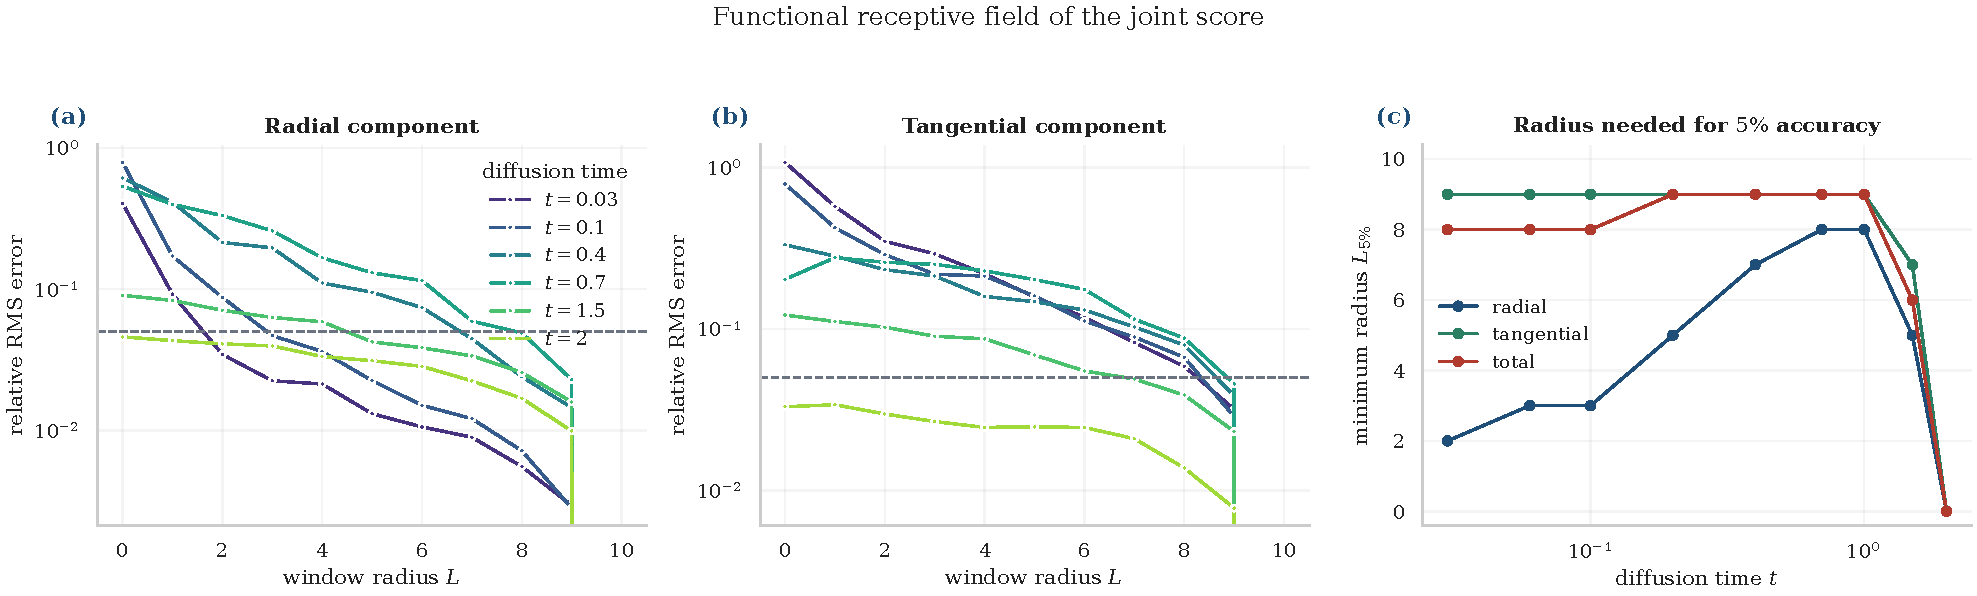
\includegraphics[width=\textwidth]{fig16_receptive_field.pdf}
\caption{Window approximation of the joint score. (a,b) Relative RMS error of the windowed
score against window radius, by channel; the dashed line is $5\%$. (c) The minimum radius
$L_{5\%}$ needed for each channel. The radial score needs a radius of $2$ at $t=0.03$ but $8$
at $t=0.7$; the tangential score needs almost the whole trajectory at low noise, and nothing
at all by $t=2$.}
\label{fig:receptive-field}
\end{figure}

At $t=0.03$ the radial component of the score reaches $5\%$ accuracy with a window radius of
$2$, while the tangential component needs $9$ --- nearly the whole trajectory. At intermediate
diffusion times both channels need large windows. By $t=2$ a single frame is already within
$5\%$ of the full score, because the cross-frame correction has become negligible; the
required radius is $0$. This is the same non-monotonicity as in the surrogate, and it is the
diagnostic with the most direct implication for architecture: the useful temporal receptive
field of a denoiser is a function of the noise level, and it is largest in the middle of the
schedule.

\subsection{The clean dynamics control the low-noise reach}

\begin{figure}[H]
\centering
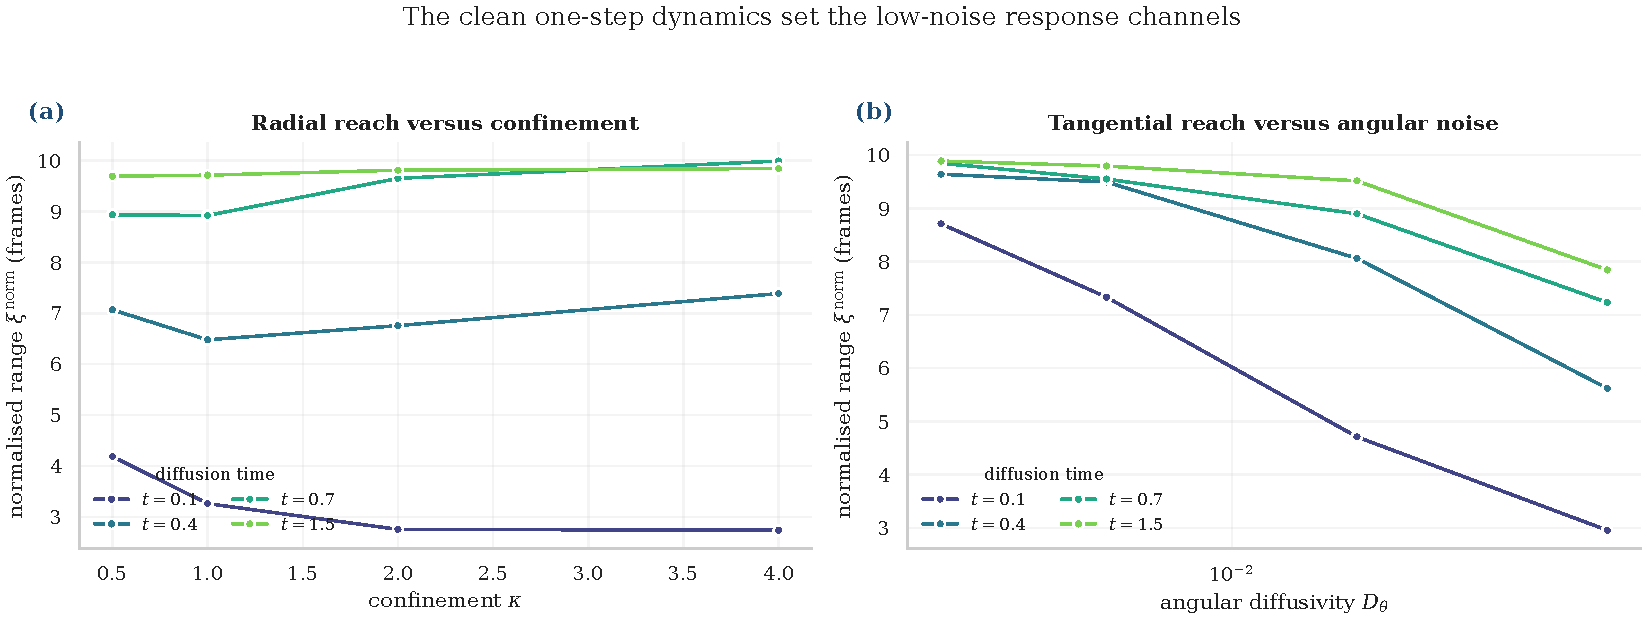
\includegraphics[width=0.9\textwidth]{fig17_parameter_sweeps.pdf}
\caption{Sweeping the clean parameters. Stronger radial confinement $\kappa$ shortens the
radial reach; larger angular diffusivity $D_\theta$ shortens the tangential reach. At large
diffusion time both curves are pushed towards the finite-size ceiling regardless of the
parameter.}
\label{fig:parameter-sweeps}
\end{figure}

The low-noise trends follow the clean scales of \cref{sec:analytic-reach}. Increasing $\kappa$
from $0.5$ to $4$ at $t=0.1$ shortens the radial normalised range $\xi^{\mathrm{norm}}_r$ from
$4.18$ to $2.74$ frames and reduces the nearest-neighbour radial intensity by an order of
magnitude, from $0.35$ to $0.034$: stiffer confinement forgets faster. Increasing $D_\theta$
from $0.002$ to $0.08$ at the same diffusion time shortens $\xi^{\mathrm{norm}}_\theta$ from
$8.71$ to $2.96$ frames:
faster dephasing destroys the long tangential channel. Both are what
\eqref{eq:gamma-r}--\eqref{eq:linear-angular-cov} predict, and together they are the concrete
answer to the research question --- the reach of the noised score is set by the one-step clean
kernel, modulated by the observation precision $\lambda_t$.

\section{Numerical validation}\label{sec:validation}

Every identity used above is checked against an independently computed reference.

\begin{table}[H]
\centering
\caption{Validation summary. The full report is in \texttt{validation.json}.}
\label{tab:validation}
\begin{tabular}{@{}lrr@{}}
\toprule
check & discrepancy & tolerance \\
\midrule
posterior covariance vs finite differences (polar) & $6.63\times10^{-9}$ & $1.00\times10^{-7}$ \\
analytic surrogate Jacobian vs finite differences & $9.18\times10^{-6}$ & $1.00\times10^{-4}$ \\
$41\times128$ vs $51\times192$ response grid & $3.04\times10^{-11}$ & $1.00\times10^{-7}$ \\
rotation gauge round trip & $2.22\times10^{-16}$ & $1.00\times10^{-12}$ \\
clean score on an exact co-rotating ring path & $0$ (exact) & $1.00\times10^{-12}$ \\
\bottomrule
\end{tabular}

\end{table}

\begin{figure}[H]
\centering
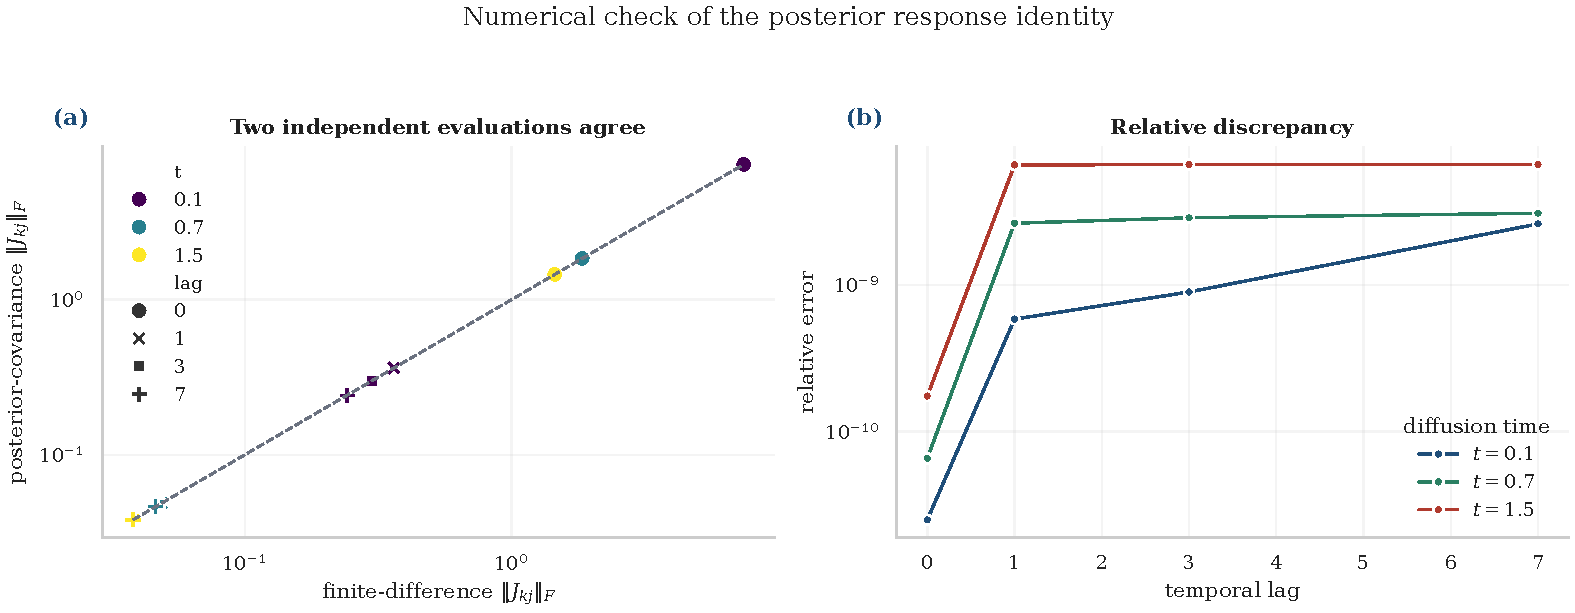
\includegraphics[width=0.92\textwidth]{fig18_validation.pdf}
\caption{The response identity \eqref{eq:fdt} evaluated two ways: from posterior pair
covariances, and by central finite differences of the score after perturbing $x_j$. (a) The
two agree along the diagonal. (b) Relative discrepancies stay below $6.7\times10^{-9}$ in the
cases tested.}
\label{fig:fdt-validation}
\end{figure}

\begin{table}[H]
\centering
\caption{First-order Taylor score against the nonlinear grid score. The central-block error
has a floor of $3$--$4\%$ from the estimated reference phase; the growth beyond $t\approx0.7$
follows the angular posterior spread (\cref{sec:taylor-validity}).}
\label{tab:taylor}
\begin{tabular}{@{}rrrr@{}}
\toprule
$t$ & central RMSE & trajectory RMSE & mean cosine \\
\midrule
0.03 & 0.039 & 0.122 & 0.985 \\
0.15 & 0.035 & 0.044 & 0.997 \\
0.40 & 0.035 & 0.035 & 0.998 \\
0.70 & 0.032 & 0.035 & 0.999 \\
1.00 & 0.061 & 0.065 & 0.992 \\
1.50 & 0.079 & 0.083 & 0.990 \\
2.00 & 0.060 & 0.067 & 0.991 \\
\bottomrule
\end{tabular}

\end{table}

Beyond the table, the checks include row normalisation of the transition kernels, global
rotation equivariance of the score, stability under halving the finite-difference step, and
the exact vanishing of the clean surrogate score on a perfect co-rotating ring path
(\cref{sec:surrogate-score}, point~2).

One caveat on grid convergence. The difference between the $41\times128$ and $51\times192$
response grids is $3\times10^{-11}$, which is small because the baseline likelihoods and
kernels are already very smooth at those resolutions. A deliberately coarse $11\times24$ grid
does show visible deviations, so the production grid is not trivially grid-independent; it is
converged for these parameters.

% ============================================================================
\section{What the experiment answers}\label{sec:answers}
% ============================================================================

\subsection{How Markovity helps, and how it does not}

The clean law is local, $p_0(h_{0:T-1})=p_0(h_0)\prod_kM(h_{k+1}\given h_k)$, and this gives
three concrete advantages: the clean score is assembled from adjacent transition innovations
(\cref{eq:clean-radial-score,eq:clean-angular-score}); the noised posterior can be integrated
by repeated one-step operators instead of one integral over $2T$ latent variables
(\cref{eq:forward-recursion,eq:backward-recursion}); and any distant influence on $S_k$ must
propagate through a sequence of local transitions, which is why the parameter sweeps of
\cref{sec:measurements} can predict the reach from the one-step kernel.

What clean Markovity does \emph{not} give is locality of the noised score. For $t>0$,
\[
 S_k(x,t)\ne F_t(x_{k-1},x_k,x_{k+1})
\]
in either model: integrating out uncertain latent states creates posterior correlations at
every lag. In the surrogate this is explicit --- the rank-one anchor term of
\eqref{eq:surrogate-jac} touches every pair of frames --- and in the polar model it is
measured.

\subsection{The mechanism, in one line}

Both models show the same sequence,
\begin{equation}
 \text{strictly local clean score}
 \;\longrightarrow\;
 \text{broader noised posterior dependence}
 \;\longrightarrow\;
 \text{weak universal field }-x .
\end{equation}
At intermediate diffusion times individual frames are noisy enough that distant context
improves the estimate of a clean frame. At large diffusion times the same context is still
statistically present but no longer materially useful, because the prefactor
$\mt^2/\Dt^2$ in \eqref{eq:fdt} has gone to zero.

\subsection{The radial--tangential separation}

The polar process shows something the Cartesian surrogate cannot express: radial information
is damped by mean reversion, while tangential information rides a slowly diffusing global
phase. The two score channels therefore have different reaches and different receptive fields,
predicted at low noise by $\xi_r^{\mathrm{clean}}=1/(\kappa h)$ and
$\xi_\theta^{\mathrm{clean}}=1/(D_\theta h)$ and confirmed by the sweeps.

\begin{keyresult}[Answer to the research question]
The clean Markov dynamics are exploited not by assuming that the noised score is local, but by
identifying the local channels through which information propagates. The cross-frame response
of the joint score is a posterior covariance \eqref{eq:fdt}; its radial and tangential decay
scales are controlled by the one-step kernel through
\eqref{eq:gamma-r}--\eqref{eq:linear-angular-cov}; and its practical receptive field depends on
the diffusion time and is largest in the middle of the schedule. In the model and parameters
studied here, tangential context is almost global near the data while radial context is
initially local, and diffusion broadens both normalised profiles while weakening their
absolute intensity until the score becomes effectively framewise again.
\end{keyresult}

% ============================================================================
\section{Limitations and next steps}\label{sec:limitations}
% ============================================================================

\begin{enumerate}
\item \textbf{One parameter set.} Every number reported here comes from a single baseline, with
      $T=20$ (polar) or $T=30$ (surrogate) and $28$--$36$ trajectories per diffusion time.
      Only $\kappa$ and $D_\theta$ were swept. Nothing is claimed about scaling in $T$.
\item \textbf{Angular equation.} We used a constant angular drift. The board admits other
      readings; a different angular drift changes the transition kernel but not the score
      identities of \cref{sec:object}.
\item \textbf{Radius positivity.} The shifted OU process \eqref{eq:shifted-radial} is formally
      supported on all of $\R$. At the baseline the probability of a negative radius is
      negligible, but a strict model would reflect at the origin or use a positive diffusion.
\item \textbf{Known rotation.} The gauge reduction of \cref{sec:gauge} assumes $\psi$ known.
      An unknown clockwise/counter-clockwise class would add a discrete latent variable and may
      produce a genuine speciation phenomenon of the kind discussed in
      \cref{sec:statmech-tools}. This is the most interesting single extension.
\item \textbf{Finite trajectory.} At large $t$ the reach diagnostics saturate at their
      structureless ceilings. This is a finite-size effect, and is not evidence of a divergent
      correlation length.
\item \textbf{Oracle projections.} The radial and tangential channels were separated using the
      simulated clean angle. A practical method would infer the phase, and the resulting error
      would enter the projected profiles.
\item \textbf{Grid approximation.} The polar score is numerically converged for these
      parameters, but it is not a symbolic closed form.
\item \textbf{One tangent plane.} The Taylor model cannot represent wrapped or multimodal
      angular posteriors, which by \cref{sec:taylor-validity} is the regime beyond
      $t\approx0.55$.
\end{enumerate}

The immediate extensions are to vary $T$ systematically, to infer the angular phase rather
than use an oracle basis, to add an unknown rotation class, and to test whether a
time-dependent local architecture with receptive field $L_\epsilon(t)$ can match the full
score.

% ============================================================================
\appendix
\section{The anchor posterior in polar form}\label{app:anchor}
% ============================================================================

This appendix records, for reproducibility only, the one-dimensional integrals the code uses
to tabulate \eqref{eq:anchor-moments}. Nothing in the main argument depends on them.

Align the first axis with $h$ and write $a=r(\cos\theta,\sin\theta)$, $\dd a=r\dd r\dd\theta$,
so that $h\T a=\rho r\cos\theta$ with $\rho=\|h\|$. The four angular integrals needed are
standard integral representations of the modified Bessel functions $I_\nu$:
\begin{align}
 \int_0^{2\pi}\e^{\rho r\cos\theta}\dd\theta&=2\pi I_0(\rho r),
 &\int_0^{2\pi}\cos\theta\,\e^{\rho r\cos\theta}\dd\theta&=2\pi I_1(\rho r),\\
 \int_0^{2\pi}\cos^2\theta\,\e^{\rho r\cos\theta}\dd\theta&=\pi\big[I_0+I_2\big](\rho r),
 &\int_0^{2\pi}\sin^2\theta\,\e^{\rho r\cos\theta}\dd\theta&=\pi\big[I_0-I_2\big](\rho r).
\end{align}
With $w(r)=\exp[-(r-1)^2/2\lambda-\beta r^2/2]$ they give
\begin{equation}
 \mu(\rho)=\frac{\int_0^\infty r^2w(r)I_1(\rho r)\dd r}
                {\int_0^\infty r\,w(r)I_0(\rho r)\dd r},
\end{equation}
and the parallel and perpendicular second moments follow from the third and fourth integrals,
after which
$\Cov(A\given x)=v_\perp I_2+(v_\parallel-v_\perp)\ohat h\ohat h\T$. All radial integrals are
evaluated by Gauss--Legendre quadrature, with the exponential rescaled to avoid overflow.

% ============================================================================
\section{The exact wrapped angular score}\label{app:wrapped}
% ============================================================================

With $G_q(\delta)=\sum_{n\in\mathbb Z}\exp[-(\delta+2\pi n)^2/2q]$,
\begin{equation}
 s_q(\delta)=\frac{G_q'(\delta)}{G_q(\delta)}
 =-\frac{\sum_n(\delta+2\pi n)\exp[-(\delta+2\pi n)^2/2q]}
        {q\sum_n\exp[-(\delta+2\pi n)^2/2q]} .
\end{equation}
This is periodic and smooth across the branch cut at $\pm\pi$. When $q$ is small and $\delta$
is away from $\pm\pi$, the nearest winding dominates and $s_q(\delta)\approx-\delta/q$, which
is the linear-Gaussian score used in \eqref{eq:phi-rw}.

% ============================================================================
\section{Reproduction}\label{app:repro}
% ============================================================================

From the bundle root:
\begin{lstlisting}[language=bash]
python code/compute_surrogate_full_windows.py   # window sweep for the surrogate
python code/make_tables.py                      # all LaTeX tables from data/
python code/make_figures.py                     # all figures
python code/validate.py                         # numerical checks -> validation.json
tectonic -X compile main.tex                    # or latexmk -pdf main.tex
\end{lstlisting}
The curated CSV files under \texttt{data/} are the canonical numerical outputs; the heavier
scripts that produced them are preserved as \texttt{code/run\_*\_original.py}. No number in
the text or tables is entered by hand: \texttt{code/make\_tables.py} regenerates every table
from \texttt{data/} and \texttt{validation.json}, and \texttt{code/metrics.py} contains the
single definition of the diagnostics of \cref{sec:diagnostics}.

\paragraph{Simulation provenance.}
\begin{table}[H]
\centering\small
\begin{tabularx}{\textwidth}{@{}lX@{}}
\toprule
Study & Main settings \\
\midrule
Surrogate, exact & $T=30$, $\lambda=0.05$, $\sigma=0.15$, $350$ trajectories,
  quadrature anchor posterior \\
Polar, response & $T=20$, $\kappa=2$, $D_r=0.015$, $D_\theta=0.005$, $41\times128$ grid,
  $28$ trajectories per diffusion time \\
Polar, windows & $36$ trajectories per diffusion time, radii $L=0,\ldots,10$ \\
Taylor comparison & $32$ trajectories per diffusion time; reference phase estimated by
  de-rotating and averaging the noisy frames \\
Angular posterior spread & $6$ trajectories per diffusion time, $41\times128$ grid \\
Score-field figures & one fixed clean trajectory and one fixed standardised noise realisation,
  $31\times64$ grid \\
\bottomrule
\end{tabularx}
\end{table}

% ============================================================================
\begingroup
\small
\begin{thebibliography}{99}
\setlength{\itemsep}{0.2em}

\bibitem[Abramson et al.(2024)]{abramson2024alphafold3}
J. Abramson et al.
\newblock Accurate structure prediction of biomolecular interactions with AlphaFold~3.
\newblock \emph{Nature} 630:493--500, 2024.

\bibitem[Achilli et al.(2026)]{achilli2026speciation}
B. Achilli, M. Benedetti, G. Biroli, and M. M\'ezard.
\newblock Theory of speciation transitions in diffusion models with general class structure.
\newblock arXiv:2602.04404, 2026.

\bibitem[Anderson(1982)]{anderson1982reverse}
B. D. O. Anderson.
\newblock Reverse-time diffusion equation models.
\newblock \emph{Stochastic Processes and their Applications} 12(3):313--326, 1982.

\bibitem[Bachtis et al.(2024)]{bachtis2024cascade}
D. Bachtis, G. Biroli, A. Decelle, and B. Seoane.
\newblock Cascade of phase transitions in the training of energy-based models.
\newblock \emph{Advances in Neural Information Processing Systems} 37, 2024.

\bibitem[Biroli et al.(2024)]{biroli2024dynamical}
G. Biroli, T. Bonnaire, V. De Bortoli, and M. M\'ezard.
\newblock Dynamical regimes of diffusion models.
\newblock arXiv:2402.18491, 2024.

\bibitem[Einstein(1905)]{einstein1905brownian}
A. Einstein.
\newblock \"Uber die von der molekularkinetischen Theorie der W\"arme geforderte Bewegung von
in ruhenden Fl\"ussigkeiten suspendierten Teilchen.
\newblock \emph{Annalen der Physik} 322(8):549--560, 1905.

\bibitem[It\^o(1944)]{ito1944stochastic}
K. It\^o.
\newblock Stochastic integral.
\newblock \emph{Proceedings of the Imperial Academy of Tokyo} 20:519--524, 1944.

\bibitem[Landau and Lifshitz(1980)]{landau1980statistical}
L. D. Landau and E. M. Lifshitz.
\newblock \emph{Statistical Physics, Part 1}.
\newblock Pergamon, 3rd edition, 1980.

\bibitem[Langevin(1908)]{langevin1908theorie}
P. Langevin.
\newblock Sur la th\'eorie du mouvement brownien.
\newblock \emph{Comptes Rendus de l'Acad\'emie des Sciences} 146:530--533, 1908.

\bibitem[M\'ezard(2025)]{mezardnotes}
M. M\'ezard.
\newblock Generative diffusion: updated notes.
\newblock Lecture notes, December 2025.

\bibitem[M\'ezard and Montanari(2009)]{mezard2009information}
M. M\'ezard and A. Montanari.
\newblock \emph{Information, Physics, and Computation}.
\newblock Oxford University Press, 2009.

\bibitem[Rombach et al.(2022)]{rombach2022latent}
R. Rombach, A. Blattmann, D. Lorenz, P. Esser, and B. Ommer.
\newblock High-resolution image synthesis with latent diffusion models.
\newblock \emph{IEEE/CVF Conference on Computer Vision and Pattern Recognition}, 2022.

\bibitem[Sclocchi et al.(2025)]{sclocchi2025phase}
A. Sclocchi, A. Favero, and M. Wyart.
\newblock A phase transition in diffusion models reveals the hierarchical nature of data.
\newblock \emph{Proceedings of the National Academy of Sciences}, 2025. arXiv:2402.16991.

\bibitem[Sohl-Dickstein et al.(2015)]{sohl2015deep}
J. Sohl-Dickstein, E. Weiss, N. Maheswaranathan, and S. Ganguli.
\newblock Deep unsupervised learning using nonequilibrium thermodynamics.
\newblock \emph{International Conference on Machine Learning}, 2015. arXiv:1503.03585.

\bibitem[Song et al.(2021)]{song2021scorebased}
Y. Song, J. Sohl-Dickstein, D. P. Kingma, A. Kumar, S. Ermon, and B. Poole.
\newblock Score-based generative modeling through stochastic differential equations.
\newblock \emph{International Conference on Learning Representations}, 2021.

\bibitem[Uhlenbeck and Ornstein(1930)]{uhlenbeck1930theory}
G. E. Uhlenbeck and L. S. Ornstein.
\newblock On the theory of the Brownian motion.
\newblock \emph{Physical Review} 36:823--841, 1930.

\end{thebibliography}
\endgroup

\end{document}
